% ============================================================
%  BÁO CÁO ĐỒ ÁN — Nhập môn Khoa học Dữ liệu (IT4930)
%  Trường Đại học Bách khoa Hà Nội — SOICT
%  Compile: XeLaTeX
% ============================================================
\documentclass{article}
\usepackage{fontspec}
\setmainfont{TeX Gyre Termes}
\setsansfont{TeX Gyre Heros}
\setmonofont{DejaVu Sans Mono}
\usepackage{amsmath}
\usepackage{graphicx}
\usepackage{amssymb}
\usepackage{geometry}
\geometry{a4paper, margin=1in}
\usepackage{hyperref}
\usepackage{booktabs}
\usepackage{fancyhdr}
\usepackage{listings}
\usepackage[vietnamese]{babel}

\addto\captionsvietnamese{
  \renewcommand{\contentsname}{Mục lục}
  \renewcommand{\listfigurename}{Danh sách Hình}
  \renewcommand{\listtablename}{Danh sách Bảng}
  \renewcommand{\refname}{Tài liệu tham khảo}
  \renewcommand{\abstractname}{Tóm tắt}
  \renewcommand{\figurename}{Hình}
  \renewcommand{\tablename}{Bảng}
}

\usepackage{tabularx}
\usepackage{multirow}
\usepackage{array}
\usepackage{longtable}
\newcolumntype{L}[1]{>{\raggedright\arraybackslash}m{#1}}
\newcolumntype{C}[1]{>{\centering\arraybackslash}m{#1}}
\newcolumntype{R}[1]{>{\raggedleft\arraybackslash}m{#1}}

\usepackage{float}
\usepackage{subcaption}
\usepackage{caption}
\captionsetup{font=small, labelfont=bf, labelsep=period, justification=centering}
\graphicspath{{images/}}

\usepackage{setspace}
\onehalfspacing

\lstset{
  basicstyle        = \ttfamily\small,
  frame             = single,
  breaklines        = true,
  showstringspaces  = false,
  xleftmargin       = 4pt,
  xrightmargin      = 4pt,
}

\usepackage{enumitem}
\usepackage{parskip}
\usepackage{pifont}
\setlength{\parindent}{0pt}
\setlength{\parskip}{5pt}

\hypersetup{
  colorlinks = true,
  linkcolor  = black,
  citecolor  = black,
  urlcolor   = black,
  pdftitle   = {Báo cáo Đồ án IT4930 — Giá thuê Nhà trọ/Căn hộ},
  pdfauthor  = {Nhóm IT4930 HUST}
}

\pagestyle{fancy}
\fancyhf{}
\fancyhead[L]{\small\textit{IT4930 — Phân tích \& dự báo giá thuê Nhà trọ/Căn hộ}}
\fancyhead[R]{\small\textit{HUST 2025.2}}
\fancyfoot[C]{\small\thepage}
\renewcommand{\headrulewidth}{0.4pt}

% ─────────────────────────────────────────────────────────────
\begin{document}


\begin{titlepage}
\begin{center}
    \textbf{ĐẠI HỌC BÁCH KHOA HÀ NỘI} \\
    \textbf{TRƯỜNG CÔNG NGHỆ THÔNG TIN VÀ TRUYỀN THÔNG} \\
    \vspace{0.2cm}
\end{center}

\begin{figure}[htbp]
    \centering
    
\includegraphics[width=0.6\textwidth]{soict_logo.jpg}
\end{figure}

\begin{center}
    \Large \textbf{PHÂN TÍCH \& DỰ BÁO GIÁ THUÊ NHÀ TRỌ / CĂN HỘ THEO KHU VỰC} \\
    \vspace{0.4cm}
    \normalsize \textit{Đồ án môn Nhập môn Khoa học Dữ liệu (IT4142)} \\
    \vspace{1.5cm}

    \begin{tabular}{|c|l|l|}
        \hline
        \textbf{STT} & \textbf{Họ và tên} & \textbf{Mã số sinh viên} \\
        \hline
        1 & Nguyễn Xuân Sơn  & 20235823 \\
        \hline
        2 & Nguyễn Phạm Gia Phát    & 20235805 \\
        \hline
        3 & Văn Thành Đạt   & 20235677 \\
        \hline
        4 & Nguyễn Mạnh Quyền  & 20235820 \\
        \hline
        5 & Nguyễn Danh Dũng   & 20235685 \\
        \hline
        6 & Trịnh Thành An    & 20235633 \\
        \hline
        7 & Nguyễn Mạnh Đức    & 20235681 \\
        \hline
        8 & Nguyễn Hồng Dương    & 20235693 \\
        \hline
    \end{tabular}

    \vspace{1cm}

    \begin{tabular}{ll}
        \textbf{Giảng viên hướng dẫn:} & TS. Nguyễn Đức Anh \\[0.4cm]
        \textbf{Học kỳ:}               & 2025.2            \\[0.4cm]
        % \textbf{Ngày nộp:}             & Tháng 6, 2025     \\
    \end{tabular}

\end{center}

\vspace{2cm}
\end{titlepage}
\clearpage


\tableofcontents
\newpage
% \listoffigures
% \listoftables
\newpage

% ── CẤU TRÚC 6 PHẦN (theo cautrucbaocao.md) ──────────────────────
% 1. Giới thiệu (Motivation)
% 2. Các nghiên cứu / giải pháp đã có (Related Works)
% 3. Dữ liệu & Bài toán ban đầu (Data Pipeline + EDA)
% 4. Phương pháp (Methodology: formalize + cũ→đề xuất)
% 5. Kịch bản đánh giá & Kết quả (CV + Test + Ablation)
% 6. Kết luận (Summary + Lessons + Future work)
%    + Tài liệu tham khảo (cuối báo cáo)
% ─────────────────────────────────────────────────────────────────
%% ============================================================
%%  SECTION 1 — GIỚI THIỆU (Introduction)
%%  Trả lời: Tại sao lại chọn đề tài này? (Motivation)
%% ============================================================
\section{Giới thiệu}
\label{sec:intro}

\subsection{Động lực và tính cấp thiết}

Thị trường cho thuê nhà trọ và căn hộ tại Việt Nam đang phát triển mạnh,
đặc biệt tại các đô thị lớn như Hà Nội và TP. Hồ Chí Minh.
Tuy nhiên, thông tin giá thuê hiện nằm rải rác trên hàng chục trang web với định dạng
và đơn vị không thống nhất; không ít tin đăng chỉ ghi \textit{``giá thỏa thuận''},
khiến người thuê khó so sánh và đánh giá mức giá hợp lý.

Vấn đề này tạo ra ba hướng giá trị thực tiễn mà đồ án hướng tới:
\begin{enumerate}[leftmargin=*, itemsep=3pt]
  \item \textbf{Đối với người thuê:} có thể ước lượng mức giá tham khảo hợp lý
        trước khi đàm phán, tránh bị định giá quá cao.
  \item \textbf{Đối với chủ nhà:} hiểu được mặt bằng khu vực để định giá cạnh tranh.
  \item \textbf{Đối với nghiên cứu:} cung cấp bộ dữ liệu tổng hợp đa nguồn đầu tiên
        về thị trường cho thuê Việt Nam, cùng quy trình tái tạo công khai.
\end{enumerate}

\subsection{Ý nghĩa học thuật}

Từ góc độ Khoa học Dữ liệu, đề tài này bao trùm toàn bộ vòng đời
\textit{Knowledge Discovery in Databases} (KDD): thu thập $\to$ tích hợp $\to$ làm sạch
$\to$ khám phá (EDA) $\to$ mô hình hóa $\to$ triển khai, đặt trọng tâm vào
\textbf{chất lượng dữ liệu} và \textbf{phân tích nhân quả} thay vì chỉ tối ưu chỉ số mô hình.
Hai phát hiện điển hình là \textbf{Nghịch lý Simpson} do cấu trúc nguồn gây ra
(đòi hỏi phân tích phân tầng trước khi kết luận) và việc \textbf{kiểm toán nguồn gốc
dữ liệu} (data provenance) phát hiện 7/12 cờ tiện ích bị \textit{chế tác} ở bước tích hợp —
dẫn tới cơ chế xử lý thiếu-không-ngẫu-nhiên (MNAR) và ràng buộc đơn điệu
cho mô hình triển khai (Mục~\ref{subsec:audit}).

\subsection{Phạm vi bài toán}

\begin{itemize}[leftmargin=*, itemsep=3pt]
  \item \textbf{Input:} diện tích, số phòng ngủ/tắm, thành phố/quận, 12 cờ tiện ích.
  \item \textbf{Output:} giá thuê dự báo (số thực, triệu VNĐ/tháng)
        $\Rightarrow$ \textbf{bài toán Hồi quy}.
  \item \textbf{Phương pháp đánh giá:} MAE, RMSE, R\textsuperscript{2}
        (xem Mục~\ref{sec:eval} để biết cách thiết lập thực nghiệm).
  \item \textbf{Dữ liệu:} 133.586 bản ghi từ 10 nguồn, sau tích hợp và lọc ngoại lệ
        (Mục~\ref{sec:data}).
\end{itemize}

\subsection{Đóng góp chính}

\begin{enumerate}[leftmargin=*, itemsep=3pt]
  \item Xây dựng pipeline thu thập và tích hợp dữ liệu cho thuê đa nguồn
        (10 trang web + bộ dữ liệu công khai).
  \item Phát hiện và phân tích \textbf{Nghịch lý Simpson} do thiên lệch nguồn,
        dẫn tới quyết định thiết kế mô hình có căn cứ.
  \item Thực hiện \textbf{3 thực nghiệm đối sánh} (ablation study) kiểm chứng
        các quyết định tiền xử lý: Feature Engineering vs.\ dữ liệu thô,
        biến mục tiêu gốc vs.\ log-transform, và tác động của ngoại lệ.
  \item \textbf{Kiểm toán sau triển khai} (Mục~\ref{subsec:audit}): truy vết hành vi
        phi lý của mô hình về tận dữ liệu gốc, phát hiện \textbf{7/12 cờ tiện ích bị điền
        ngẫu nhiên} ở bước tích hợp; khắc phục bằng cơ chế \textbf{mask MNAR}
        (thiếu-không-ngẫu-nhiên) và \textbf{ràng buộc đơn điệu}, bảo đảm mô hình
        triển khai hợp lý về kinh tế học (thêm tiện ích không làm giảm giá dự báo).
  \item Triển khai ứng dụng web demo (Streamlit) dự báo giá theo khu vực.
\end{enumerate}

%% ============================================================
%%  SECTION 2 — CÁC NGHIÊN CỨU LIÊN QUAN (Related Works)
%%  Nguồn: Paper, GitHub, Kaggle, Medium
%%  Mỗi nghiên cứu: nguồn dữ liệu + phương pháp tốt nhất (SotA)
%%  Mục tiêu: xây dựng baseline + xác định khoảng trống (research gap)
%% ============================================================
\section{Các nghiên cứu / giải pháp đã có}
\label{sec:related}

\subsection{Các nghiên cứu quốc tế về dự báo giá bất động sản}

\subsubsection*{Mô hình Hedonic Pricing (nền tảng lý thuyết)}

Phương pháp \textbf{Hedonic Pricing} \cite{rosen1974hedonic} coi giá bất động sản là hàm
của tập hợp đặc điểm vật lý và vị trí: $P = f(\text{diện tích, phòng, khu vực, tiện ích}, \ldots)$.
Đây là nền tảng lý thuyết được hầu hết các nghiên cứu dự báo giá áp dụng,
trong đó OLS là mô hình baseline cổ điển nhất.
\textbf{Nguồn dữ liệu:} dữ liệu giao dịch nhà đất từ địa chính/môi giới.
\textbf{Hạn chế:} giả định quan hệ tuyến tính, nhạy cảm với đa cộng tuyến và ngoại lệ.

\subsubsection*{Kaggle — Ames Housing Dataset}

Bộ dữ liệu Ames Iowa (De Cock, 2011)~\cite{decock2011ames} với 2.930 giao dịch và 80 đặc trưng
đã trở thành chuẩn mực (benchmark) cho bài toán dự báo \textbf{giá mua bán} nhà.
Các giải pháp top Kaggle sử dụng \textbf{XGBoost/LightGBM + Feature Engineering} đạt
RMSE $\approx$ 0.10--0.12 (log-scale).
\textbf{Khoảng trống:} bộ dữ liệu này về giá mua bán (không phải cho thuê), một thành phố nhỏ
của Mỹ, và số lượng bản ghi hạn chế.

\subsubsection*{Nghiên cứu ML đa mô hình cho thị trường cho thuê}

Yılmaz \& Yakut (2022)~\cite{yilmaz2022rental} so sánh OLS, Ridge, LASSO, Random Forest và
Gradient Boosting trên dữ liệu cho thuê nhà ở Thổ Nhĩ Kỳ (12.000 bản ghi).
Kết quả: \textbf{Gradient Boosting đạt R\textsuperscript{2} $\approx$ 0.82} trên dữ liệu
một thành phố có địa chỉ chính xác (GPS).
\textbf{Phương pháp tốt nhất hiện tại (SotA):} Gradient Boosting kết hợp
đặc trưng vị trí không gian (tọa độ GPS, khoảng cách tới trung tâm).

\subsection{Các nghiên cứu / dự án về thị trường Việt Nam}

\subsubsection*{Dự án GitHub về giá nhà TP. Hồ Chí Minh}

Một số dự án mã nguồn mở trên GitHub~\cite{github_hcm_housing} thu thập dữ liệu bất động sản
TP.HCM từ batdongsan.com.vn và áp dụng Random Forest / XGBoost.
\textbf{Nguồn dữ liệu:} 2.000--8.000 bản ghi, chủ yếu TP.HCM, chú trọng giá \textbf{mua bán}.
\textbf{Kết quả điển hình:} R\textsuperscript{2} $\approx$ 0.70--0.75 (có đặc trưng GPS).
\textbf{Hạn chế:} quy mô nhỏ, một thành phố, không bao gồm thị trường \textbf{cho thuê}.

\subsubsection*{Kaggle — Vietnam Housing Dataset}

Một số bộ dữ liệu trên Kaggle về nhà đất Việt Nam (2.000--10.000 bản ghi) được cộng đồng
sử dụng để so sánh thuật toán, nhưng chủ yếu tập trung vào \textbf{giá mua bán}
và không bao gồm thông tin tiện ích chi tiết hay dữ liệu đa tỉnh thành.

\subsection{Khoảng trống nghiên cứu (Research Gap)}

\begin{table}[H]
  \centering
  \caption{So sánh nghiên cứu hiện có và đồ án này}
  \label{tab:gap}
  \small
  \begin{tabularx}{\textwidth}{@{}L{3.8cm} C{1.8cm} C{2.0cm} C{2.2cm} C{3.0cm}@{}}
    \toprule
    \textbf{Nghiên cứu} &
    \textbf{Loại thị trường} &
    \textbf{Quy mô} &
    \textbf{Phạm vi địa lý} &
    \textbf{Phương pháp tốt nhất} \\
    \midrule
    Ames Housing (Kaggle) &
      Mua bán & 2.930 & 1 thành phố & XGBoost + FE \\
    Yılmaz \& Yakut (2022) &
      Cho thuê & 12.000 & 1 thành phố & Gradient Boosting + GPS \\
    Dự án GitHub VN &
      Mua bán & $<$10.000 & TP.HCM & Random Forest \\
    \midrule
    \textbf{Đồ án này} &
      \textbf{Cho thuê} & \textbf{133.586} & \textbf{19 tỉnh/thành} &
      XGBoost + FE đa nguồn \\
    \bottomrule
  \end{tabularx}
\end{table}

\textbf{Khoảng trống mà đồ án này lấp đầy:}
\begin{itemize}[leftmargin=*, itemsep=3pt]
  \item Chưa có nghiên cứu nào về thị trường \textbf{cho thuê} quy mô lớn đa tỉnh
        tại Việt Nam (hầu hết tập trung vào mua bán hoặc một thành phố).
  \item Không có pipeline \textbf{tích hợp đa nguồn} (10 nguồn) với lược đồ thống nhất
        và xử lý chất lượng dữ liệu có hệ thống.
  \item Chưa có phân tích kiểm chứng quyết định thiết kế bằng \textbf{thực nghiệm đối sánh}
        (ablation study) công khai cho bài toán giá thuê Việt Nam.
\end{itemize}

%% ============================================================
%%  SECTION 3 — DỮ LIỆU & BÀI TOÁN BAN ĐẦU  (số liệu: v2)
%%  Data Pipeline: thu thập → tích hợp → làm sạch → EDA → Final Data
%% ============================================================
\section{Dữ liệu và Bài toán ban đầu}
\label{sec:data}

\subsection{Lý do chọn bộ dữ liệu}

Không có bộ dữ liệu cho thuê đa nguồn sẵn có ở Việt Nam,
nên nhóm tự thu thập bằng \textbf{web scraping} từ 10 nguồn khác nhau.
Lý do chọn cách này:
\begin{itemize}[leftmargin=*, itemsep=2pt]
  \item Bao phủ nhiều phân khúc thị trường (từ phòng trọ bình dân tới căn hộ).
  \item Đảm bảo tính đại diện địa lý (Hà Nội, TP.HCM, Đà Nẵng và 16 tỉnh thành khác).
  \item Có thể kiểm soát chất lượng và schema từ đầu, thay vì phụ thuộc nguồn
        bên thứ ba có thể thay đổi.
\end{itemize}

\subsection{Thu thập dữ liệu (Web Scraping)}
\label{subsec:collection}

\begin{table}[H]
  \centering
  \caption{Phân bố bản ghi theo nguồn dữ liệu (sau làm sạch)}
  \label{tab:sources}
  \begin{tabular}{@{}lrr@{}}
    \toprule
    \textbf{Nguồn} & \textbf{Số bài} & \textbf{Tỷ lệ} \\
    \midrule
    chothuephongtro     & 95.086 & \textbf{71.2\%} \\
    nhatot              &  9.920 & 7.4\% \\
    chothuenhadattoanvn &  9.866 & 7.4\% \\
    github\_hcm         &  8.771 & 6.6\% \\
    github\_hn          &  2.879 & 2.2\% \\
    phongtro123         &  2.663 & 2.0\% \\
    github\_housing     &  1.635 & 1.2\% \\
    lozido              &  1.313 & 1.0\% \\
    facebook            &    772 & 0.6\% \\
    github\_dn          &    681 & 0.5\% \\
    \midrule
    \textbf{Tổng} & \textbf{133.586} & \textbf{100\%} \\
    \bottomrule
  \end{tabular}
\end{table}

\begin{figure}[H]
  \centering
  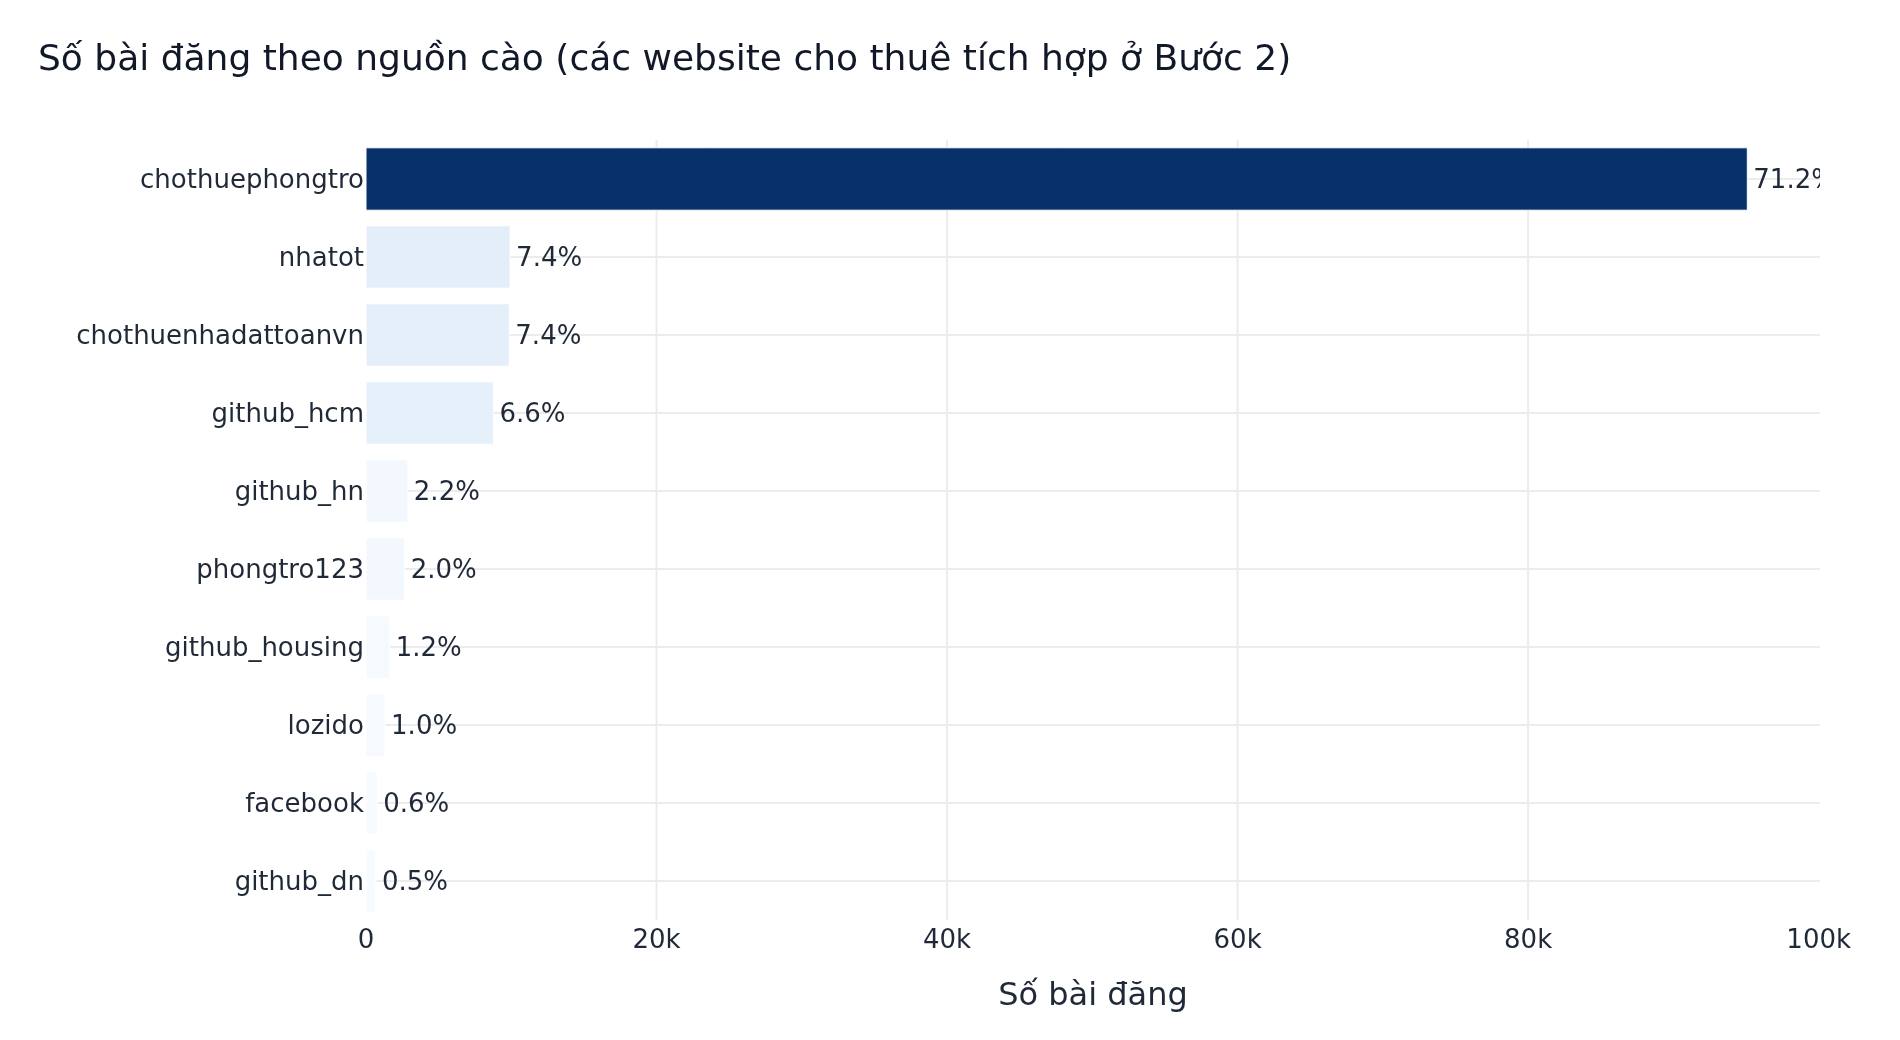
\includegraphics[width=0.86\textwidth]{eda_01_source_distribution}
  \caption{Phân bố bản ghi theo nguồn — \texttt{chothuephongtro} chiếm 71.2\%
           (mất cân bằng nghiêm trọng, quyết định loại \texttt{source} khỏi đặc trưng mô hình,
           xem Mục~\ref{subsec:simpson})}
  \label{fig:source_dist}
\end{figure}

\subsection{Tích hợp và lược đồ chung}
\label{subsec:schema}

Để hợp nhất 10 nguồn có định dạng khác nhau, nhóm thiết kế
\textbf{lược đồ thống nhất} (mediated schema) với các trường:
\texttt{price, area, bedrooms, bathrooms, full\_address, posted\_date, source}
cùng 12 cờ nhị phân \texttt{feature\_*}.
Quy trình ETL gồm bốn bước:
\begin{itemize}[leftmargin=*, itemsep=2pt]
  \item Chuẩn hóa giá và diện tích từ chuỗi văn bản về số (biểu thức chính quy).
  \item Loại tin \texttt{price = -1} (\textit{``giá thỏa thuận''}).
  \item Khử trùng lặp; mã hóa one-hot 12 tiện ích.
  \item \textbf{Lọc ngoại lệ:} \texttt{price}$\leq$17 triệu/tháng;
        \texttt{area}$\leq$180 m\textsuperscript{2}
        (ngưỡng chọn từ phân tích EDA, đúng phạm vi nhà trọ/căn hộ bình dân).
\end{itemize}

\subsection{Chất lượng dữ liệu và xử lý ngoại lệ (Outlier)}
\label{subsec:quality}

\begin{table}[H]
  \centering
  \caption{Các vấn đề chất lượng dữ liệu và cách xử lý}
  \label{tab:quality}
  \begin{tabularx}{\textwidth}{@{}L{3.0cm} L{5.2cm} X@{}}
    \toprule
    \textbf{Vấn đề} & \textbf{Phát hiện} & \textbf{Xử lý \& lý do} \\
    \midrule
    Ngoại lệ cực đoan &
      Giá tới 10.000 triệu/tháng ($\approx$10 tỷ); diện tích tới 1.000 m\textsuperscript{2} &
      Lọc \texttt{price}$\leq$17; \texttt{area}$\leq$180 — ngoại lệ kéo lệch
      hàm mất mát bình phương, làm mô hình phân bổ năng lực sai vùng giá
      (xác nhận bằng thực nghiệm~\ref{subsec:abl_outlier}) \\
    \addlinespace
    Giá trị thiếu &
      \texttt{detail\_link} 96.4\%;\newline
      \texttt{description} 80.4\%;\newline
      \texttt{district} 2.2\% (2.938 dòng) &
      Loại hai cột thiếu nhiều;\newline
      \texttt{district} thiếu $\to$ gán nhãn \textit{(không rõ)} \\
    \addlinespace
    Sentinel ngày &
      \texttt{posted\_date}: \textbf{46\%} bản ghi mang ngày tương lai &
      Không dùng \texttt{posted\_date} trong mô hình \\
    \addlinespace
    Cờ tiện ích chế tác &
      Kiểm toán raw$\leftrightarrow$hợp nhất (Mục~\ref{subsec:audit}): chỉ \textbf{5/12 cờ}
      có cột gốc thật ở đa số nguồn; 7 cờ còn lại bị \textbf{điền ngẫu nhiên} khi gộp
      ($\approx$97\% số dòng) &
      Mask các ô chế tác thành NaN theo cơ chế MNAR
      (``không khai báo'' $\neq$ ``không có'');
      loại \texttt{n\_features} khỏi đặc trưng \\
    \addlinespace
    Miền giá trị &
      Sau lọc: \texttt{price} 0.5--17;\quad \texttt{area} 8--180 &
      Hợp lệ, không cần xử lý thêm \\
    \bottomrule
  \end{tabularx}
\end{table}

\subsection{Phân tích khám phá dữ liệu (EDA)}
\label{subsec:eda}

\subsubsection*{Thống kê mô tả (Phân tích đơn biến)}

\begin{table}[H]
  \centering
  \caption{Thống kê mô tả các biến liên tục ($n = 133.586$, sau lọc ngoại lệ)}
  \label{tab:descriptive}
  \small
  \begin{tabular}{@{}lrrrrrrr@{}}
    \toprule
    \textbf{Biến} &
    \textbf{Mean} & \textbf{Std} & \textbf{Min} &
    \textbf{Median} & \textbf{Max} &
    \textbf{Skew} & \textbf{Kurt} \\
    \midrule
    \texttt{price} (tr.đ/tháng)
      & 4.80 & 2.87 & 0.5 & 4.00 & 17.0 & \textbf{1.55} & 2.46 \\
    \texttt{area} (m\textsuperscript{2})
      & 41.48 & 27.72 & 8.0 & 30.00 & 180.0 & \textbf{1.59} & 2.35 \\
    \texttt{bedrooms}
      & 1.51 & 0.98 & 0 & 1 & 6 & 2.08 & 4.45 \\
    \texttt{bathrooms}
      & 1.29 & 0.73 & 0 & 1 & 5 & 2.89 & 9.91 \\
    \texttt{n\_features}
      & 6.56 & 1.94 & 0 & 7 & 12 & $-$0.12 & $-$0.20 \\
    \bottomrule
  \end{tabular}
\end{table}

\textbf{Ý nghĩa ra quyết định:}
\texttt{price} và \texttt{area} lệch phải rõ rệt (skewness $\approx$ 1.5--1.6).
Phân phối lệch gợi ý thử log-transform; tuy nhiên thực nghiệm đối sánh
(Mục~\ref{subsec:abl_log}) cho thấy log \textbf{không} cải thiện chỉ số chính RMSE/R\textsuperscript{2}
và gây underweight phân khúc giá cao — do đó mô hình huấn luyện trên \texttt{price} gốc.

\begin{figure}[H]
  \centering
  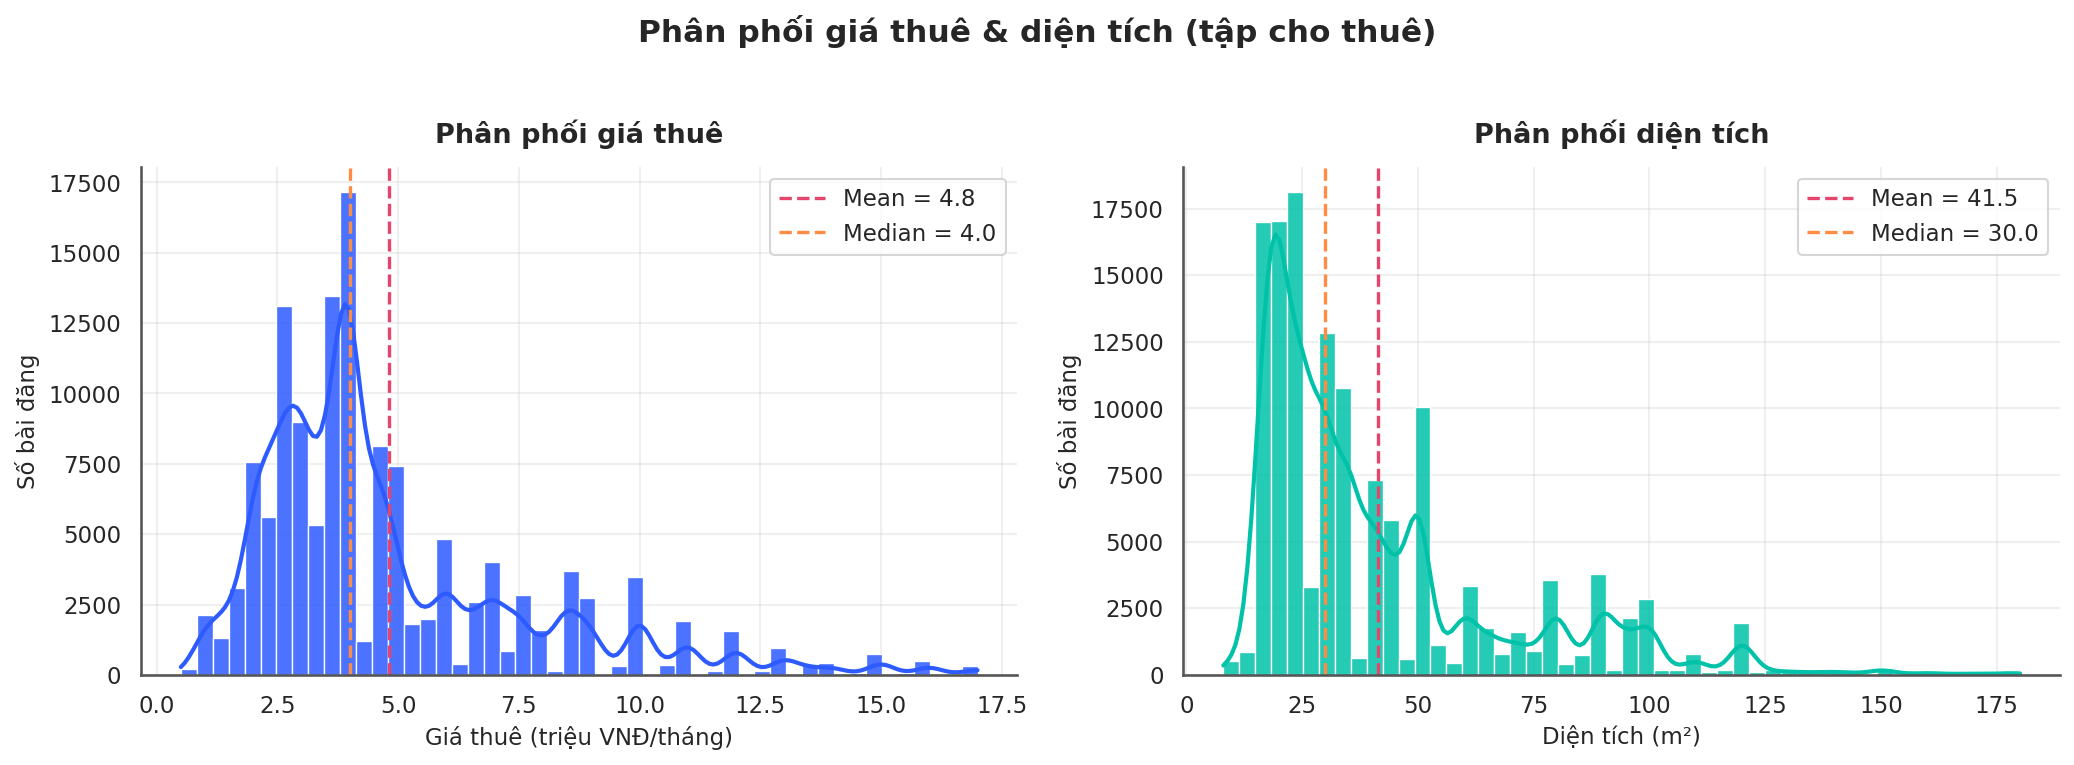
\includegraphics[width=0.86\textwidth]{eda_02_histogram_price_area}
  \caption{Phân phối \texttt{price} và \texttt{area} — cả hai lệch phải rõ rệt;
           phần lớn phòng có diện tích 20--60 m\textsuperscript{2} và giá 2--8 triệu/tháng}
  \label{fig:hist}
\end{figure}

\subsubsection*{Phân bố địa lý}

\begin{table}[H]
  \centering
  \caption{Phân bố địa lý — tập trung nặng tại Hà Nội (88\%)}
  \label{tab:geo}
  \begin{tabular}{@{}lrr@{}}
    \toprule
    \textbf{Thành phố} & \textbf{Số bài} & \textbf{Tỷ lệ} \\
    \midrule
    Hà Nội        & 117.574 & \textbf{88.0\%} \\
    Hồ Chí Minh  &  11.559 & 8.7\% \\
    Đà Nẵng      &   1.411 & 1.1\% \\
    Các tỉnh khác & $<1\%$ mỗi tỉnh & --- \\
    \bottomrule
  \end{tabular}
\end{table}

\textbf{Ý nghĩa ra quyết định:} mất cân bằng địa lý mạnh (88\% là Hà Nội).
Khi dùng One-Hot Encoding cho \texttt{district} (353 giá trị), nhiều quận tỉnh lẻ
có rất ít mẫu $\to$ cần gộp hạng mục hiếm (\texttt{min\_frequency=100}) để
tránh bùng nổ chiều và đảm bảo mô hình xử lý được hạng mục lạ lúc dự đoán.

\subsubsection*{Phân tích đa biến và tương quan}

\begin{table}[H]
  \centering
  \caption{Tương quan Spearman giữa các đặc trưng và \texttt{price}}
  \label{tab:spearman}
  \begin{tabular}{@{}lr@{}}
    \toprule
    \textbf{Biến} & \textbf{Spearman với \texttt{price}} \\
    \midrule
    \texttt{area}        & $\mathbf{+0.366}$ \\
    \texttt{bathrooms}   & $+0.141$ \\
    \texttt{bedrooms}    & $+0.115$ \\
    \texttt{n\_features} &
      $\mathbf{-0.119}$\quad\textit{(phản trực giác — xem Mục~\ref{subsec:simpson})} \\
    \bottomrule
  \end{tabular}
\end{table}

\begin{figure}[H]
  \centering
  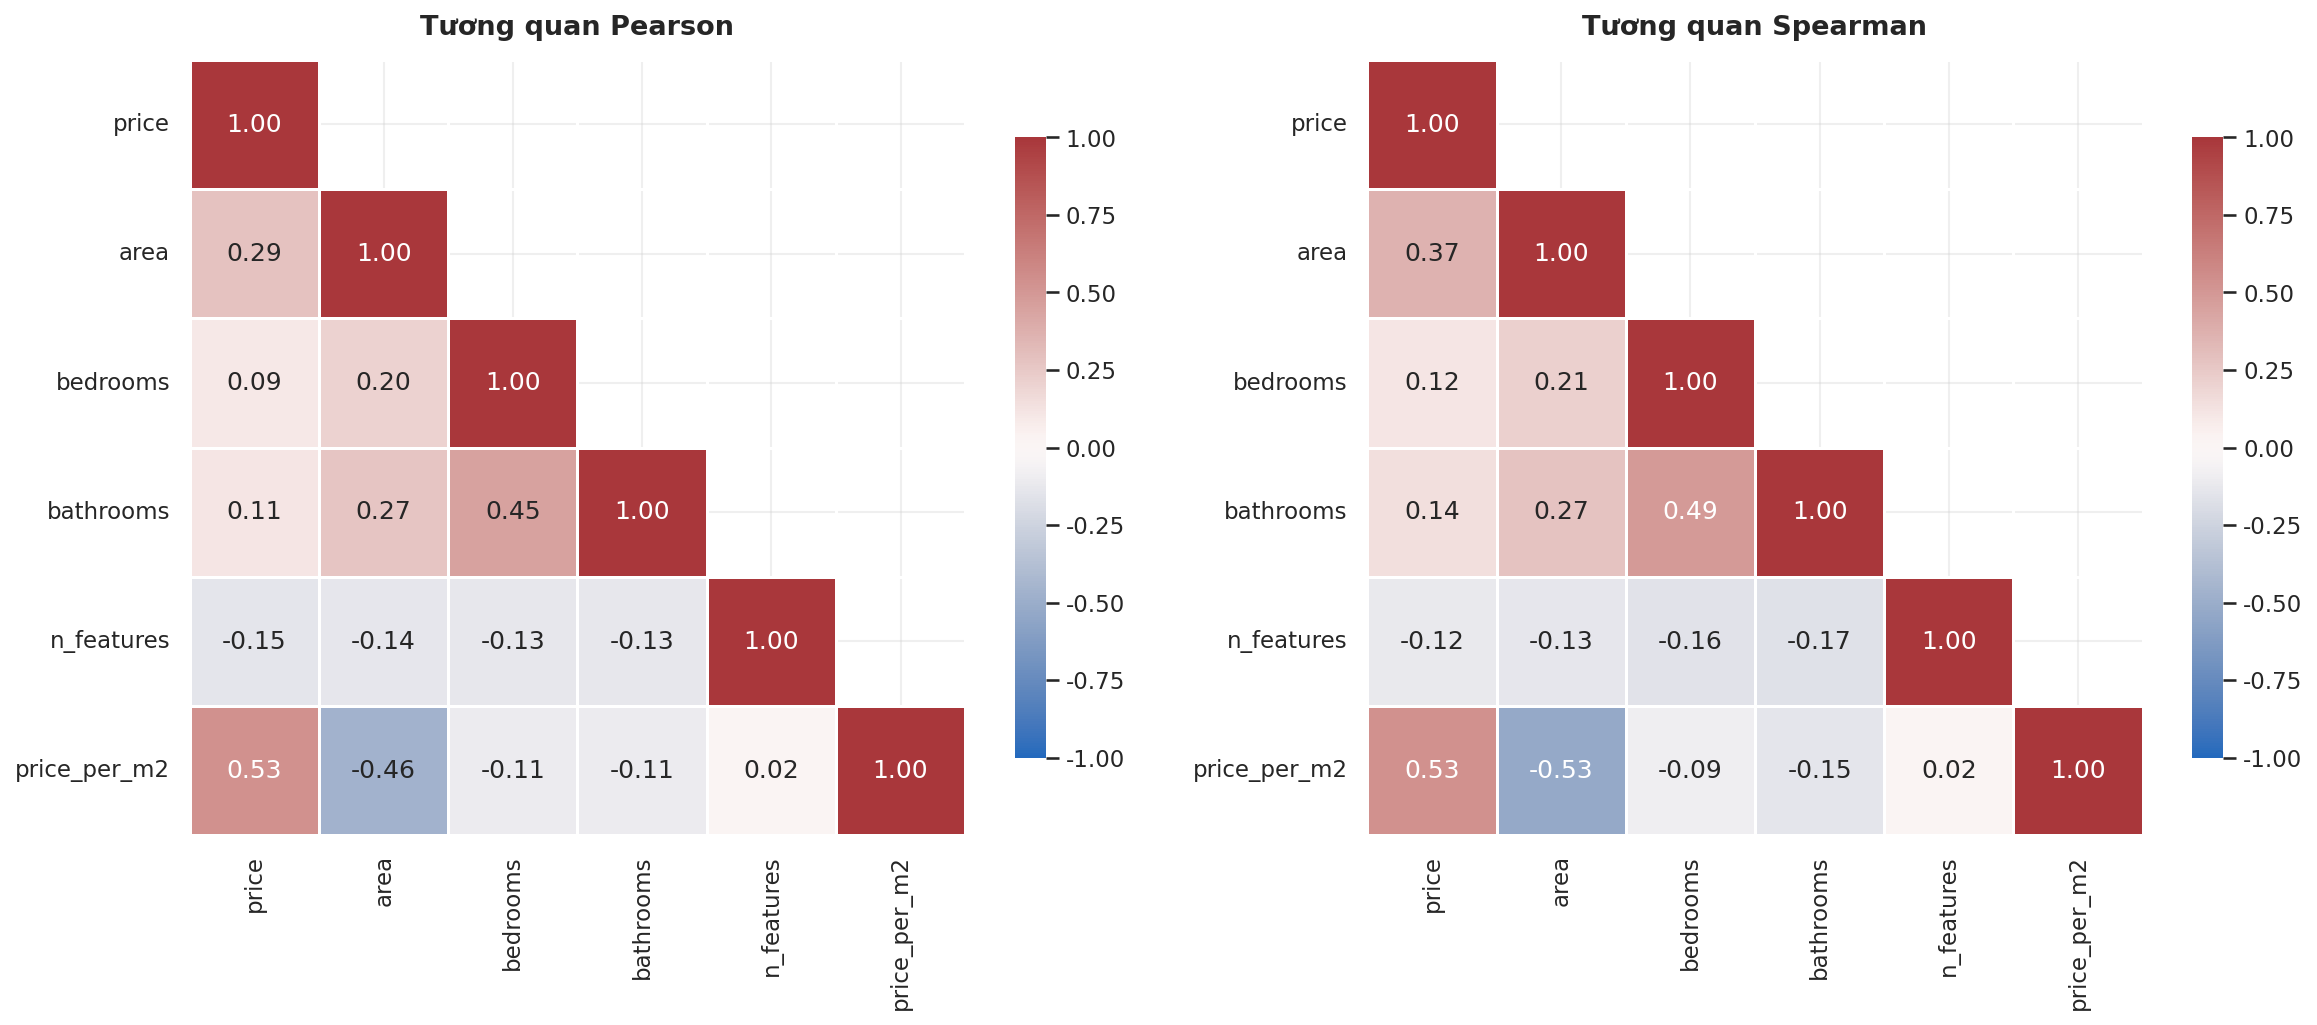
\includegraphics[width=0.76\textwidth]{eda_11_heatmap_correlation}
  \caption{Heatmap tương quan Spearman — \texttt{area} tương quan mạnh nhất với giá;
           tương quan \texttt{n\_features}--\texttt{price} âm là tín hiệu cần điều tra}
  \label{fig:heatmap}
\end{figure}

\begin{figure}[H]
  \centering
  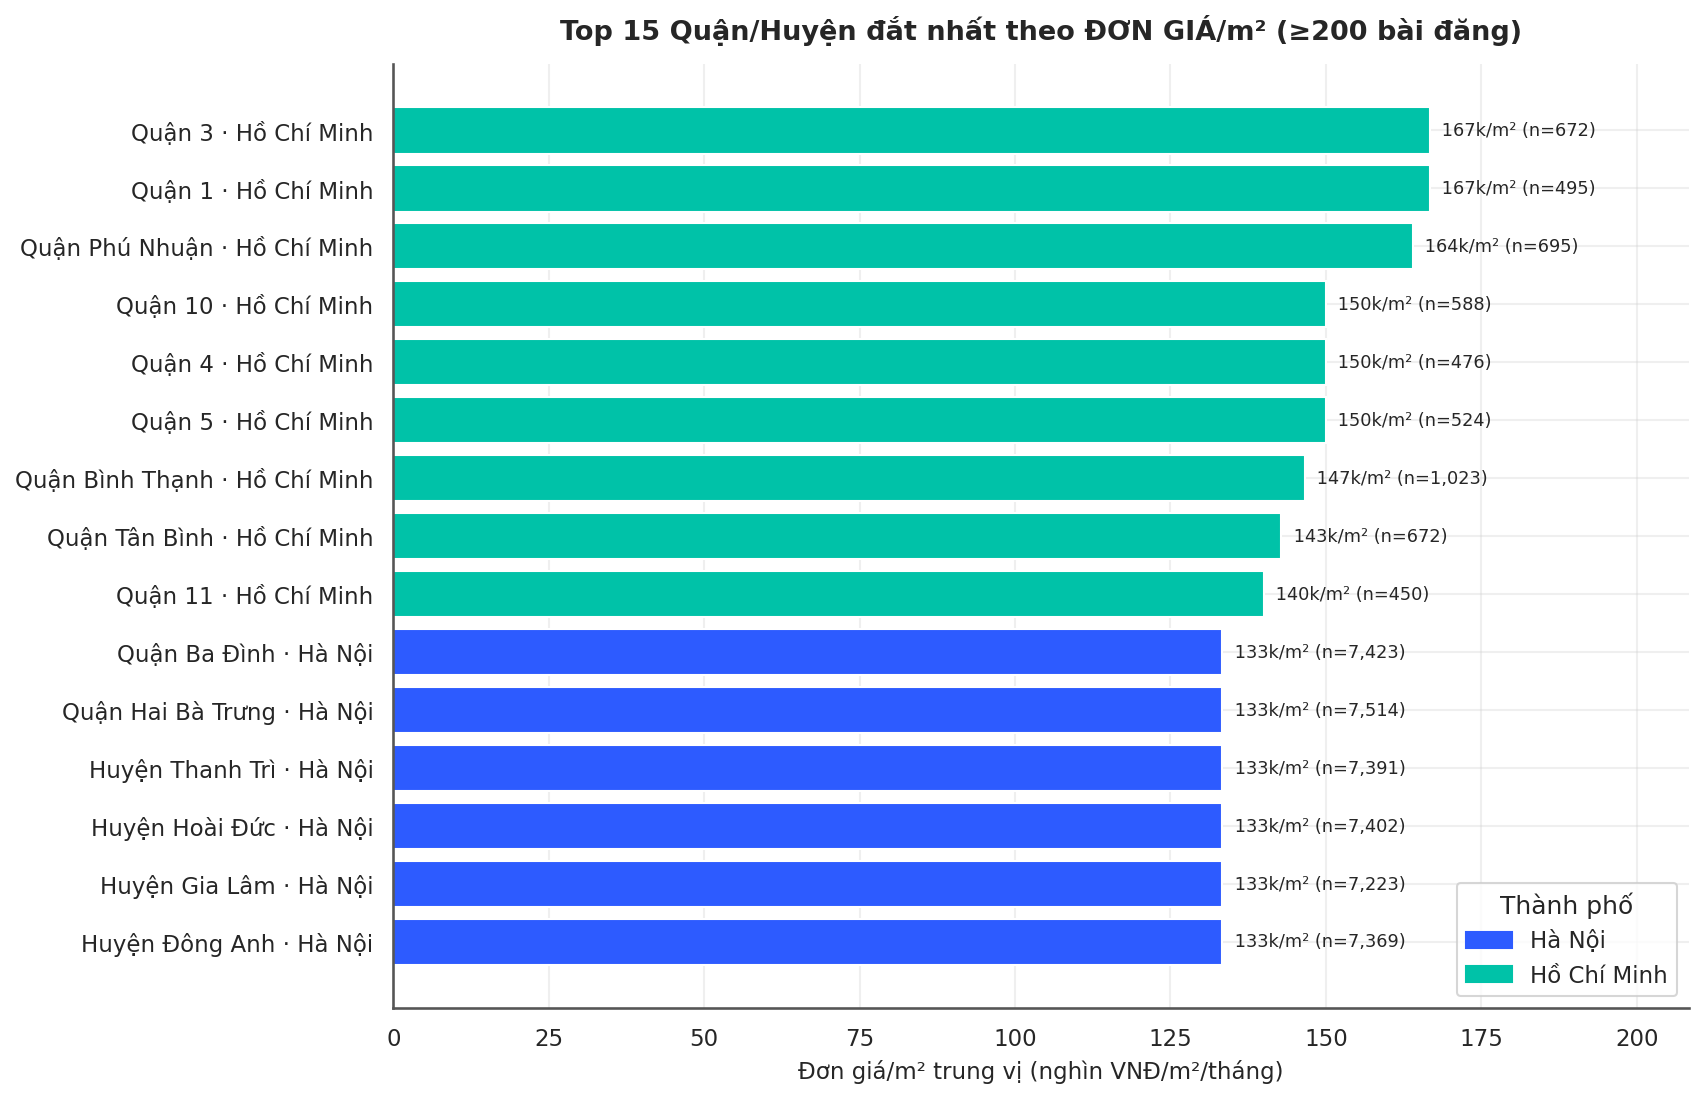
\includegraphics[width=0.86\textwidth]{eda_05_price_per_m2_ranking}
  \caption{Top quận/huyện theo đơn giá thuê — trung tâm TP.HCM (Quận 1, 3) đắt nhất;
           kết quả này thúc đẩy việc tách \texttt{city}/\texttt{district} làm đặc trưng chính}
  \label{fig:price_ranking}
\end{figure}

\subsection{Nghịch lý Simpson — phát hiện quan trọng}
\label{subsec:simpson}

\subsubsection*{Hiện tượng phản trực giác}

Khi so sánh giá trung bình giữa nhóm ``có tiện ích'' và ``không có'',
phần lớn tiện ích đi kèm với giá \textbf{thấp hơn} (bảo vệ 24/24: $-1.44$ triệu;
hầm để xe: $-1.01$; máy lạnh: $-0.73$):

\begin{figure}[H]
  \centering
  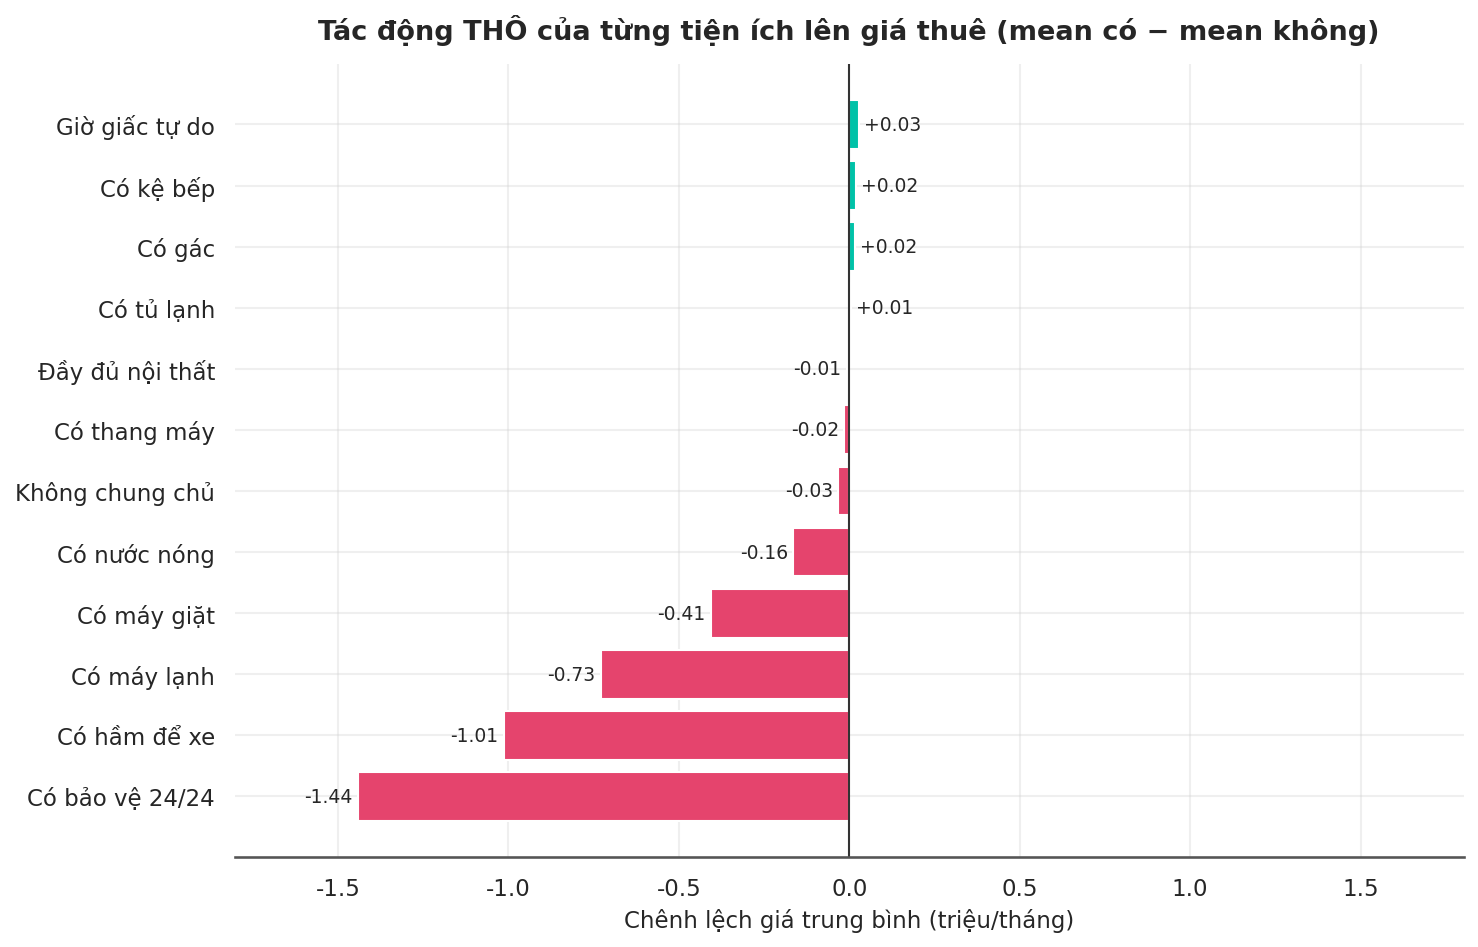
\includegraphics[width=0.86\textwidth]{eda_08_amenity_price_uplift}
  \caption{Chênh lệch giá \textbf{thô trong dữ liệu} khi có/không có từng tiện ích —
           phần lớn âm (phản trực giác). Lưu ý đây là thống kê mô tả dữ liệu như-nó-là,
           \textbf{không phải} hành vi mô hình triển khai. Câu hỏi ``tiện ích thực sự làm
           giảm giá, hay có nhân tố nhiễu?'' được trả lời từng phần ngay dưới đây
           (Nghịch lý Simpson) và triệt để ở Mục~\ref{subsec:audit}: confounding theo nguồn
           cộng với 7/12 cờ bị chế tác; mô hình triển khai cuối \textbf{không còn} hiệu ứng
           tiện ích âm nào (Hình~\ref{fig:audit_effects})}
  \label{fig:uplift}
\end{figure}

\subsubsection*{Điều tra: Nghịch lý Simpson do thiên lệch nguồn}

Kiểm tra tương quan \texttt{n\_features}--\texttt{price} \textbf{trong từng nguồn riêng biệt}:

\begin{table}[H]
  \centering
  \caption{Tương quan Spearman(\texttt{n\_features}, \texttt{price}) theo nguồn — Nghịch lý Simpson}
  \label{tab:simpson}
  \begin{tabular}{@{}lr@{}}
    \toprule
    \textbf{Nguồn} ($\geq$2.000 bài) &
    \textbf{Spearman(\texttt{n\_features}, \texttt{price})} \\
    \midrule
    phongtro123         & $\mathbf{+0.212}$ \\
    chothuenhadattoanvn & $+0.013$ \\
    github\_hn          & $-0.003$ \\
    github\_hcm         & $-0.007$ \\
    chothuephongtro     & $-0.039$ \\
    nhatot              & $-0.100$ \\
    \midrule
    \textbf{Toàn cục} & $\mathbf{-0.119}$ \\
    \bottomrule
  \end{tabular}
\end{table}

\begin{figure}[H]
  \centering
  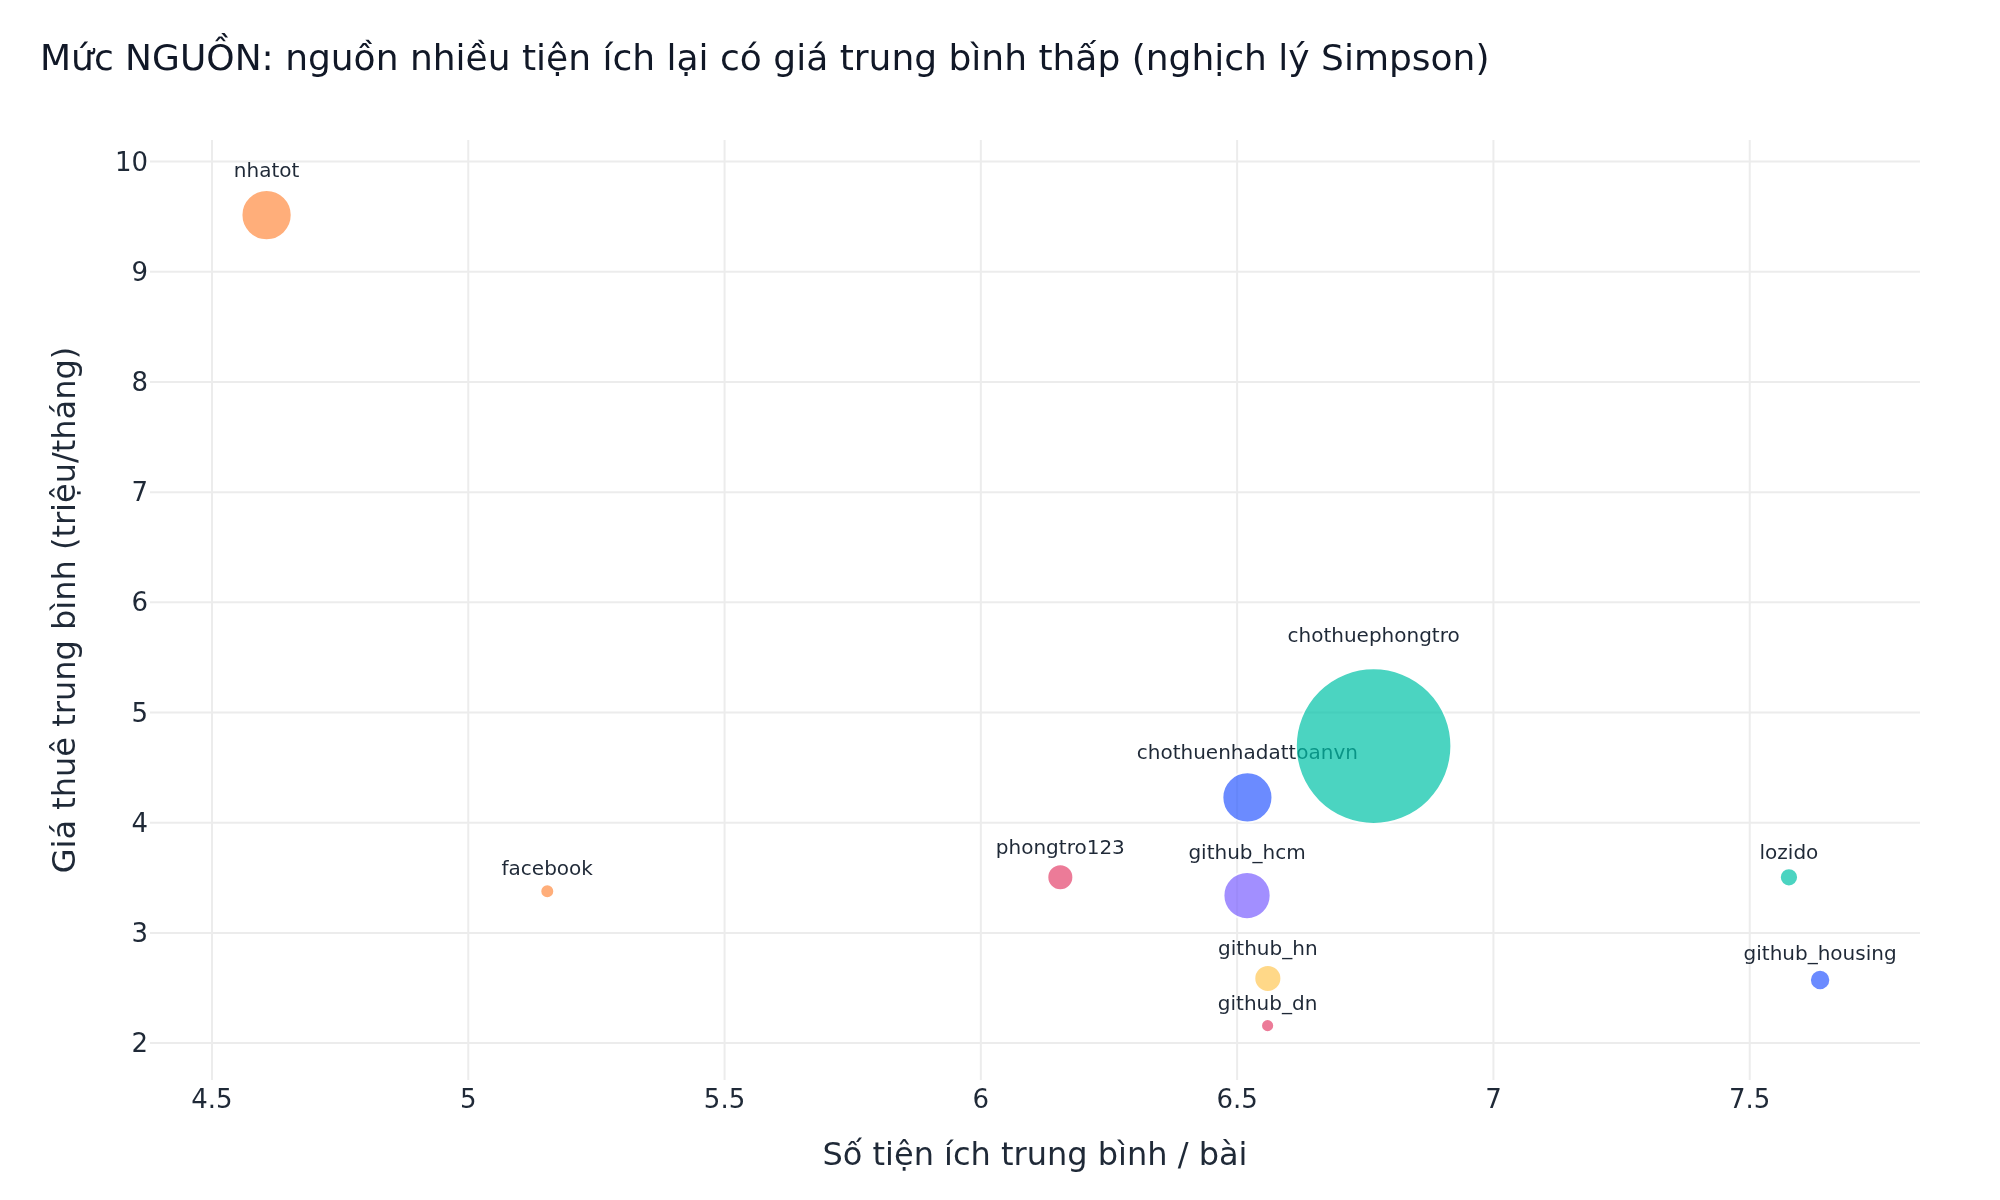
\includegraphics[width=0.86\textwidth]{eda_12_simpson_source_paradox}
  \caption{Nghịch lý Simpson: tương quan âm toàn cục do \texttt{chothuephongtro}
           (71\% dữ liệu, mặt bằng giá thấp, nhiều tiện ích) kéo trung bình xuống}
  \label{fig:simpson}
\end{figure}

\begin{quote}
  \textbf{Kết luận và quyết định thiết kế:}
  Mối tương quan âm toàn cục là do \textbf{confounding variable} — nguồn \texttt{chothuephongtro}
  chiếm 71.2\%, mặt bằng giá thấp nhưng liệt kê nhiều tiện ích.
  Hệ quả: \textbf{loại \texttt{source}} khỏi đặc trưng mô hình
  (đánh đổi một phần độ chính xác để mô hình dự báo từ đặc điểm bất động sản thật,
  không từ ``tin lấy ở web nào'').
\end{quote}

Đáng chú ý, các giá trị tương quan \textbf{gần như bằng 0 tuyệt đối} ở nhiều nguồn
(\texttt{chothuenhadattoanvn} $+0.013$, \texttt{github\_hn} $-0.003$, \texttt{github\_hcm}
$-0.007$) hóa ra là \textit{manh mối} của một vấn đề sâu hơn: kiểm toán sau triển khai
(Mục~\ref{subsec:audit}) phát hiện phần lớn cờ tiện ích của các nguồn này được
\textbf{điền ngẫu nhiên} ở bước tích hợp — biến ngẫu nhiên độc lập thì tương quan
bằng 0 với mọi thứ. Vì \texttt{n\_features} là tổng của 12 cờ trong đó 7 cờ là số
chế tác, biến này bị \textbf{loại khỏi đặc trưng mô hình} (vẫn dùng trong EDA để
mô tả dữ liệu như-nó-là).

\subsection{Feature Engineering — từ dữ liệu thô sang đặc trưng mô hình}
\label{subsec:fe}

Bước quan trọng nhất: \textbf{tách \texttt{city} và \texttt{district} từ chuỗi
\texttt{full\_address}} — đây là cách duy nhất đưa tín hiệu khu vực vào mô hình.
Thực nghiệm đối sánh (Mục~\ref{subsec:abl_fe}) xác nhận bước này là nguồn cải thiện
RMSE chính (3.5--9.4\%).

\begin{table}[H]
  \centering
  \caption{Thiết kế đặc trưng (Feature Engineering) cuối cùng — $\approx$80 chiều sau One-Hot}
  \label{tab:features}
  \begin{tabularx}{\textwidth}{@{}l X X@{}}
    \toprule
    \textbf{Nhóm} & \textbf{Đặc trưng} & \textbf{Biểu diễn} \\
    \midrule
    Số (NUM) &
      \texttt{area, bedrooms, bathrooms} &
      Chuẩn hóa Z-score
      (cần cho Ridge/LASSO; thực nghiệm~\ref{subsec:abl_fe} xác nhận) \\
    Danh mục (CAT) &
      \texttt{city, district} (tách từ \texttt{full\_address}) &
      One-Hot, gộp hạng mục hiếm (\texttt{min\_freq=100})
      $\to$ $\approx$65 chiều \\
    Nhị phân (BIN) &
      12 cờ \texttt{feature\_*} &
      0/1; ô bị chế tác $\to$ \textbf{NaN} (mask MNAR, Mục~\ref{subsec:audit}) —
      mô hình cây xử lý NaN trực tiếp, mô hình tuyến tính dùng imputer (mean) \\
    \bottomrule
  \end{tabularx}
\end{table}

\textbf{Cột bị loại có chủ đích:}
\begin{itemize}[leftmargin=*, itemsep=2pt]
  \item \texttt{source} — Nghịch lý Simpson (Mục~\ref{subsec:simpson}).
  \item \texttt{n\_features} — tổng của 12 cờ trong đó 7 cờ chế tác
        (Mục~\ref{subsec:audit}) $\Rightarrow$ phép đếm vô nghĩa,
        lại mang ``dấu vân tay nguồn''.
  \item \texttt{price\_per\_m2}, \texttt{log\_price} — rò rỉ nhãn.
  \item \texttt{posted\_date} — 46\% là giá trị sentinel.
  \item \texttt{description}, \texttt{detail\_link} — thiếu 80--96\%.
\end{itemize}

\subsection{Phân cụm K-Means và PCA}
\label{subsec:clustering}

\subsubsection*{Phân cụm K-Means ($K = 4$)}

K-Means trên (\texttt{price, area, n\_features}) chuẩn hóa, chọn $K=4$
bằng phương pháp Elbow + Silhouette.
\textbf{Ý nghĩa ra quyết định:} 4 phân khúc tương ứng với 4 đối tượng
người dùng khác nhau trong app demo (phòng bình dân, phổ thông, khá và cao cấp).

\begin{figure}[H]
  \centering
  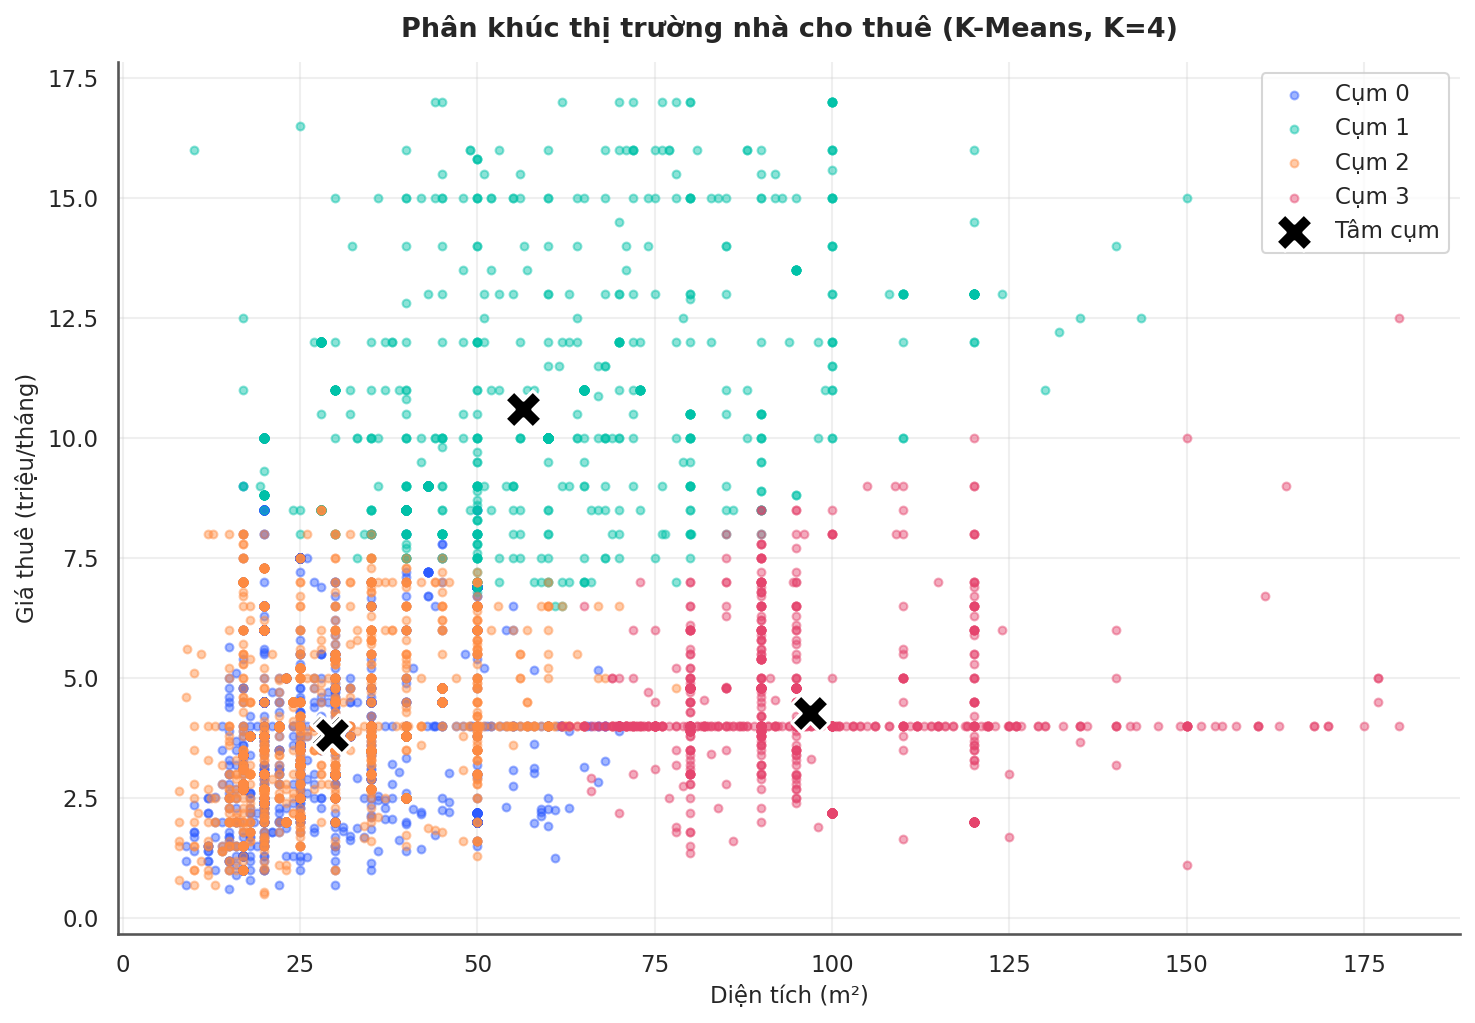
\includegraphics[width=0.86\textwidth]{eda_14_kmeans_clusters}
  \caption{4 phân khúc thị trường (K-Means, $K=4$) trên không gian
           \texttt{price} $\times$ \texttt{area}}
  \label{fig:kmeans}
\end{figure}

\subsubsection*{PCA — Cấu trúc dữ liệu}

PC1 = 36.4\%, PC2 = 21.2\%, tổng 57.6\% phương sai.
PC1 phản ánh ``quy mô'' (diện tích + số phòng + giá cùng tăng).
\textbf{Ý nghĩa:} cấu trúc tuyến tính còn lại (42.4\% phương sai chưa giải thích bởi 2 PC)
gợi ý quan hệ phi tuyến giữa khu vực và giá — lý do cần thử mô hình cây.

\begin{figure}[H]
  \centering
  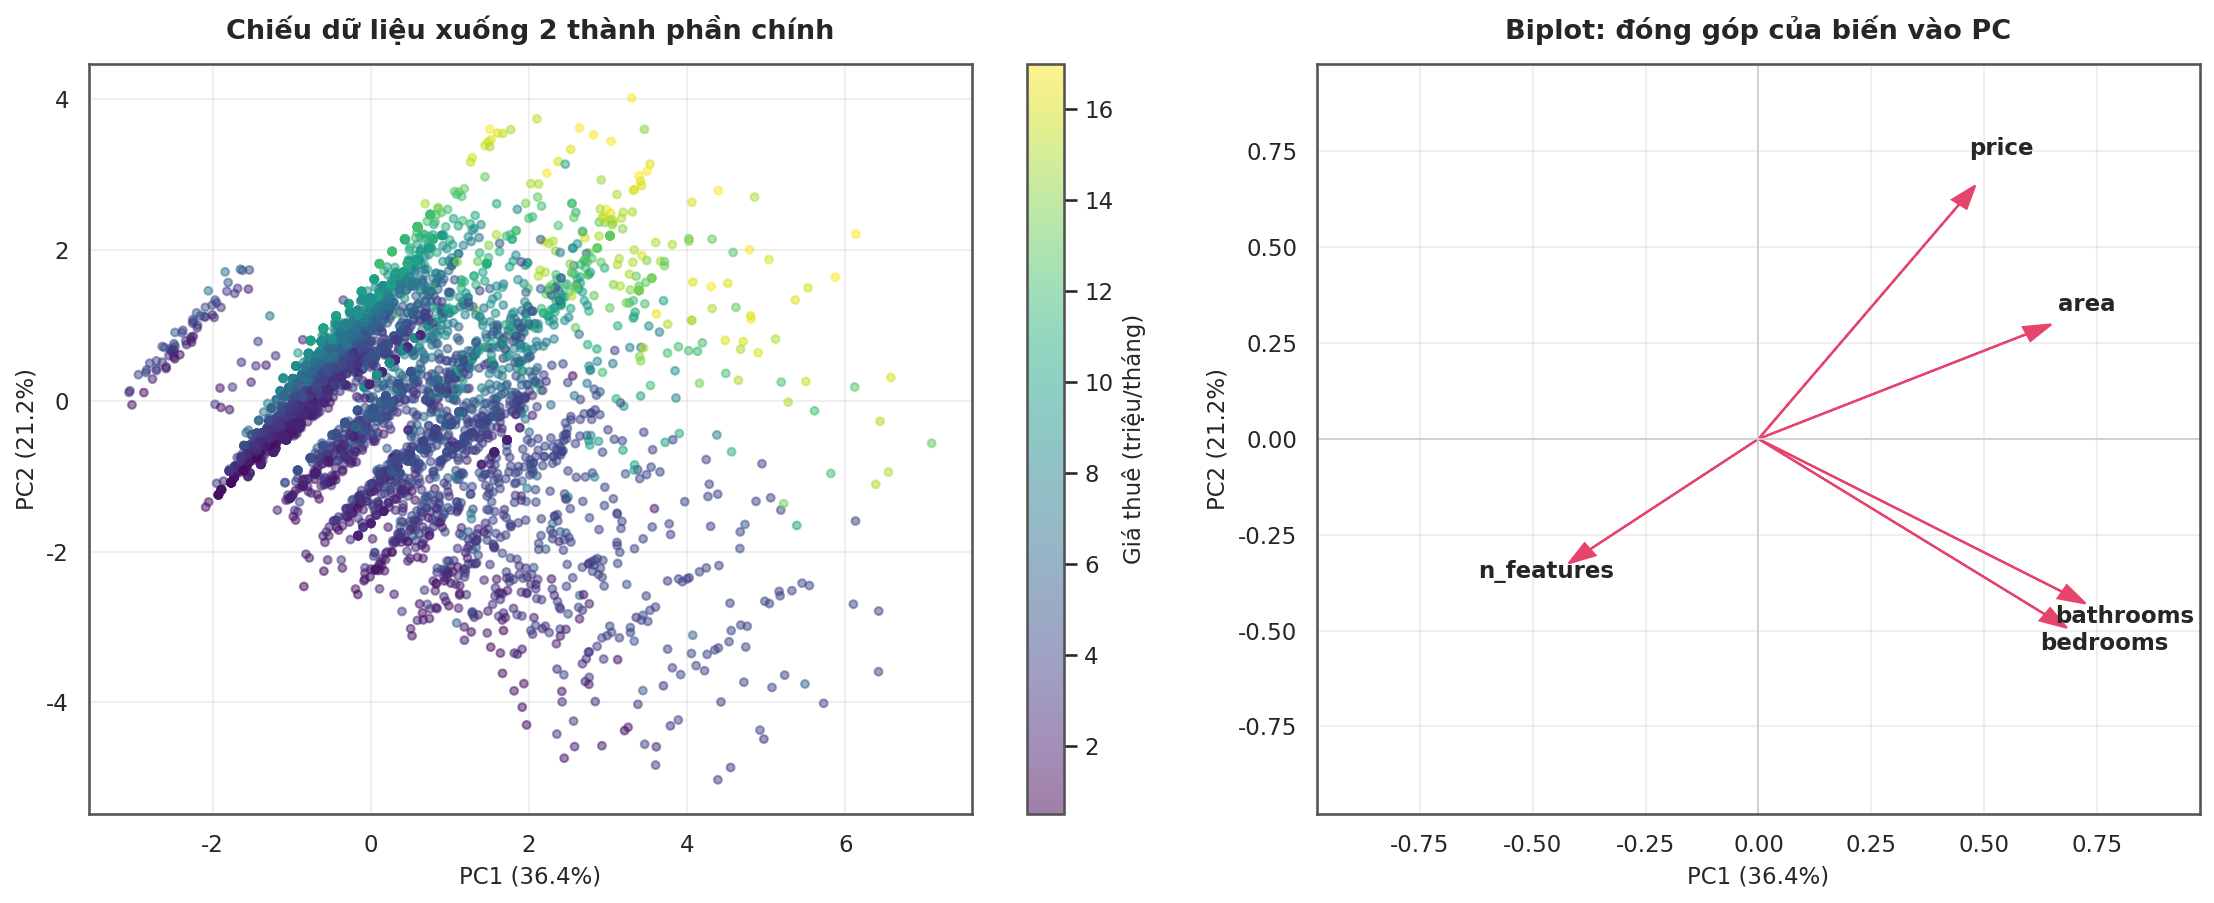
\includegraphics[width=0.80\textwidth]{eda_15_pca_2d_biplot}
  \caption{PCA 2D + Biplot: PC1 = 36.4\%, PC2 = 21.2\% — cấu trúc tuyến tính rõ nhưng
           chưa đủ giải thích toàn bộ phương sai; mô hình phi tuyến cần thiết}
  \label{fig:pca}
\end{figure}

\subsection{Bộ dữ liệu cuối (Final Data)}

Sau toàn bộ pipeline xử lý:
\begin{itemize}[leftmargin=*, itemsep=2pt]
  \item \textbf{133.586 bản ghi}; đặc trưng mô hình gồm 3 biến số + 2 biến danh mục
        (\texttt{city}/\texttt{district} tách từ FE) + 12 cờ tiện ích
        (đã mask MNAR — Bảng~\ref{tab:features}).
  \item Chia Train/Validation/Test = \textbf{70/15/15} (93.563 / 19.985 / 20.038 bản ghi).
  \item Tập Test giữ kín từ đây, chỉ dùng \textbf{đúng 1 lần} ở Mục~\ref{sec:eval}.
\end{itemize}

%% ============================================================
%%  SECTION 4 — PHƯƠNG PHÁP (Methodology)  (số liệu: v2)
%% ============================================================
\section{Phương pháp}
\label{sec:method}

\subsection{Định hình bài toán (Reformulate Problem)}
\label{subsec:formulate}

\subsubsection*{Không gian đầu vào}

Mỗi bản ghi nhà trọ/căn hộ được biểu diễn bằng vector đặc trưng
$\mathbf{x} \in \mathcal{X}$ gồm ba nhóm:

\begin{itemize}[leftmargin=*, itemsep=3pt]
  \item \textbf{Số (NUM):}
        $\mathbf{x}_\text{num} = (\text{area}, \text{bedrooms}, \text{bathrooms})
        \in \mathbb{R}^3$,
        sau chuẩn hóa Z-score: $\tilde{\mathbf{x}}_\text{num} \in \mathbb{R}^3$.
  \item \textbf{Danh mục (CAT):}
        $(\text{city}, \text{district})$, sau One-Hot Encoding với gộp hạng mục hiếm
        (\texttt{min\_freq=100}): $\mathbf{x}_\text{cat} \in \{0,1\}^{d_\text{cat}}$,
        $d_\text{cat} \approx 65$.
  \item \textbf{Nhị phân (BIN):}
        12 cờ tiện ích $\mathbf{x}_\text{bin} \in \{0, 1, \texttt{NaN}\}^{12}$
        lúc huấn luyện (\texttt{NaN} = ô bị chế tác, mask theo cơ chế MNAR —
        Mục~\ref{subsec:audit}); lúc dự đoán người dùng khai báo trực tiếp nên
        luôn là $\{0,1\}^{12}$.
\end{itemize}

Sau khi kết hợp: $\mathbf{x} \in \mathbb{R}^{d}$, $d \approx 80$.

\subsubsection*{Không gian đầu ra}

$y \in \mathbb{R}^+$ là giá thuê (triệu VNĐ/tháng).
Đây là bài toán \textbf{Hồi quy} (Regression), không phải phân loại.

\subsubsection*{Mô hình hóa}

Tìm hàm $f_\theta: \mathbb{R}^d \to \mathbb{R}^+$ cực tiểu hàm mất mát trên tập huấn luyện
$\mathcal{D}_\text{train} = \{(\mathbf{x}_i, y_i)\}_{i=1}^{N}$:

\[
  \theta^* = \arg\min_\theta \frac{1}{N}\sum_{i=1}^{N} \mathcal{L}(y_i,\, f_\theta(\mathbf{x}_i))
\]

Với hàm mất mát $\mathcal{L} = (y - \hat{y})^2$ (MSE).
Hiệu năng đo bằng:
\begin{align*}
  \text{MAE} &= \frac{1}{n}\sum|y_i - \hat{y}_i|
  \quad(\text{triệu VNĐ/tháng — dễ diễn giải thực tế}), \\
  \text{RMSE} &= \sqrt{\frac{1}{n}\sum(y_i - \hat{y}_i)^2}
  \quad(\text{phạt nặng sai số lớn — tiêu chí chọn mô hình chính}), \\
  R^2 &= 1 - \frac{\sum(y_i-\hat{y}_i)^2}{\sum(y_i-\bar{y})^2}
  \in (-\infty, 1]
  \quad(\text{tỷ lệ phương sai giải thích}).
\end{align*}

\subsection{Các phương pháp: từ baseline đến đề xuất}
\label{subsec:models}

Theo nguyên lý \textbf{No-Free-Lunch} (không có thuật toán nào tối ưu
cho mọi bài toán), nhóm thử nghiệm 5 thuật toán theo thứ tự tăng dần
về độ phức tạp — mỗi bước đều có lý do kỹ thuật cụ thể.

\subsubsection*{Phương pháp 1 (Baseline): OLS — Hồi quy tuyến tính thường}

\[
  \hat{y} = \mathbf{x}^\top\mathbf{w} + b,
  \quad \mathbf{w}^* = (\mathbf{A}^\top\mathbf{A})^{-1}\mathbf{A}^\top\mathbf{y}
\]

Nghiệm chuẩn tối thiểu RSS.
\textbf{Vai trò:} mốc tham chiếu (baseline) để đo mức cải thiện của các phương pháp sau.
\textbf{Nhược điểm đã biết:} nhạy với đa cộng tuyến (one-hot encoding $\approx$80 chiều có thể gây vấn đề);
không nắm bắt được quan hệ phi tuyến và tương tác khu vực × diện tích.

\subsubsection*{Phương pháp 2 (Cập nhật từ OLS): Ridge (L2) và LASSO (L1)}

Ridge thêm phạt L2:
$\mathbf{w}^* = \arg\min\bigl[\|\mathbf{y}-\mathbf{A}\mathbf{w}\|^2 + \lambda\|\mathbf{w}\|_2^2\bigr]$
— luôn có nghiệm duy nhất, giảm overfitting.

LASSO thêm phạt L1:
$\mathbf{w}^* = \arg\min\bigl[\|\mathbf{y}-\mathbf{A}\mathbf{w}\|^2 + \lambda\|\mathbf{w}\|_1\bigr]$
— đẩy nhiều hệ số về đúng 0, tự động chọn đặc trưng.

\textbf{Tại sao tốt hơn OLS:}
Ridge ổn định hơn khi có đa cộng tuyến; LASSO loại bỏ được các chiều One-Hot
hiếm không có tín hiệu giá (đẩy nhiều hệ số về đúng 0).
Tinh chỉnh $\alpha$ bằng GridSearchCV ($\alpha \in \{0.001, 0.01, 0.1, 1, 10, 100\}$).
Best: Ridge $\alpha = 1.0$; LASSO $\alpha = 0.001$.

\subsubsection*{Phương pháp 3 (Phi tuyến): Random Forest (Bagging)}

Tổ hợp $T$ cây quyết định huấn luyện trên bootstrap sample:
$\hat{y} = \frac{1}{T}\sum_{t=1}^{T}h_t(\mathbf{x})$.
Mỗi nút chỉ xét $\sqrt{d}$ đặc trưng ngẫu nhiên (ngẫu nhiên hóa thêm để giảm tương quan giữa cây).

\textbf{Tại sao tốt hơn tuyến tính:}
Nắm bắt được tương tác phi tuyến (khu vực × diện tích);
bagging giảm phương sai — ổn định với dữ liệu nhiễu.
Tinh chỉnh bằng RandomizedSearchCV.
Best: 200 cây, depth 10, \texttt{min\_split=5}.

\subsubsection*{Phương pháp đề xuất: XGBoost (Gradient Boosting với Regularization)}

Boosting: mỗi cây $t$ sửa residual của tổ hợp trước theo hướng gradient âm:
\[
  F_t(\mathbf{x}) = F_{t-1}(\mathbf{x}) + \eta\, h_t(\mathbf{x}),
  \quad h_t = \arg\min_h \sum_i \mathcal{L}'(y_i, F_{t-1}(\mathbf{x}_i))\cdot h(\mathbf{x}_i)
\]

Hàm mục tiêu XGBoost = loss + regularization (L1 \texttt{reg\_alpha} + L2 \texttt{reg\_lambda}).

\textbf{Tại sao chọn XGBoost để triển khai} — dù Random Forest chính xác hơn trên chỉ số thô
(Mục~\ref{subsec:main_results}), XGBoost thắng ở hai tiêu chí quan trọng hơn cho một
\textit{ứng dụng thực tế}:

\begin{table}[H]
  \centering
  \caption{So sánh Random Forest và XGBoost — vì sao triển khai XGBoost dù RF chính xác hơn}
  \label{tab:rf_vs_xgb}
  \begin{tabularx}{\textwidth}{@{}L{3.4cm} X X@{}}
    \toprule
    \textbf{Tiêu chí} & \textbf{Random Forest} & \textbf{XGBoost (triển khai)} \\
    \midrule
    Độ chính xác (Test R\textsuperscript{2}) & \textbf{0.664} & 0.565 \\
    Hành vi tiện ích & Không ràng buộc — \textbf{có hiệu ứng âm} phi lý &
      \textbf{Ràng buộc đơn điệu} — tiện ích luôn $\ge 0$ \\
    Kích thước mô hình & $\approx$5.6 MB (200 cây) & \textbf{$\approx$0.86 MB} \\
    Triển khai (GitHub <100MB, app) & Nặng hơn & \textbf{Gọn, suy luận nhanh} \\
    Kiểm soát overfitting & Bagging & Regularization + \textbf{early stopping} \\
    \bottomrule
  \end{tabularx}
\end{table}

\textbf{Ràng buộc đơn điệu (monotone constraints).} Đây là điểm then chốt khiến XGBoost phù hợp
triển khai. Kiểm toán hành vi (Mục~\ref{subsec:audit}) cho thấy nếu để tự do, mô hình học được
hiệu ứng \textit{âm} cho một số tiện ích — phi lý về kinh tế học, bắt nguồn từ confounding
``tin giá rẻ quảng cáo tiện ích, căn hộ đắt không liệt kê''. Ta áp ràng buộc đơn điệu: với mỗi
cờ tiện ích $j$, mọi cây trong tổ hợp bị ép thỏa
\[
  x_j \le x_j' \;\Rightarrow\; f_\theta(\ldots, x_j, \ldots) \le f_\theta(\ldots, x_j', \ldots),
\]
tức \textbf{tick thêm tiện ích không bao giờ làm giảm giá dự báo} (các đặc trưng khác giữ nguyên).
Nhánh ``không khai báo'' (NaN do mask MNAR) không bị ràng buộc, nên mô hình vẫn dùng được thông
tin nguồn-có-khai-báo lúc huấn luyện.

\textbf{Quy trình tinh chỉnh} (mô hình triển khai gắn ràng buộc ngay từ đầu):
(1) RandomizedSearchCV dò lưới (\texttt{lr, depth, subsample, colsample, reg\_alpha, reg\_lambda})
\textit{với ràng buộc đơn điệu trên 12 cờ tiện ích};
(2) refit cấu hình tốt nhất với \texttt{early\_stopping\_rounds=50} trên Validation
($n_\text{estimators}=2000$ làm trần; tự dừng ở \textbf{126 cây}).
Best: lr=0.05, depth=10, subsample=0.6, colsample=1.0, $\lambda=10$, $\alpha=1$.

%% ============================================================
%%  SECTION 5 — KỊCH BẢN ĐÁNH GIÁ & KẾT QUẢ  (số liệu: v2)
%% ============================================================
\section{Kịch bản đánh giá và kết quả}
\label{sec:eval}

\subsection{Thiết lập thực nghiệm}

Quy trình đánh giá tuân theo hai tầng phân tách rõ ràng:

\begin{enumerate}[leftmargin=*, itemsep=3pt]
  \item \textbf{Tầng 1 — Ablation studies (Mục~\ref{subsec:abl_fe}--\ref{subsec:abl_outlier}):}
        3 thực nghiệm đối sánh kiểm chứng từng quyết định tiền xử lý \textit{trước} khi chạy
        mô hình chính thức.
        Mục đích: xác nhận bằng số liệu (không chỉ lập luận) rằng các lựa chọn thiết kế
        là đúng đắn.
        Cùng siêu tham số đóng băng, cùng tập Validation, chỉ thay đổi \textbf{một yếu tố} mỗi lần.

  \item \textbf{Tầng 2 — Đánh giá chính thức (Mục~\ref{subsec:main_results}):}
        Sau khi các quyết định pipeline đã được xác nhận ở Tầng 1,
        5 mô hình được huấn luyện và đánh giá trên \textbf{pipeline dứt khoát}.
        \begin{itemize}[itemsep=1pt]
          \item \textbf{Model Selection:} 10-fold Cross-Validation trên Train+Val (85\%).
          \item \textbf{Model Assessment:} đánh giá \textbf{đúng 1 lần} trên Test (15\%)
                — ước lượng không thiên lệch cho hiệu năng thực tế.
        \end{itemize}

  \item \textbf{Tầng 3 — Kiểm toán sau triển khai (Mục~\ref{subsec:audit}):}
        soi hành vi của mô hình đã triển khai trong đúng kịch bản app demo
        (\textit{behavioral testing}); truy vết một hiệu ứng phi lý về tận dữ liệu gốc,
        dẫn tới phát hiện cờ tiện ích chế tác và bản vá mô hình triển khai cuối cùng.
\end{enumerate}

% ─────────────────────────────────────────────────────────────────
\subsection{Thực nghiệm A — Dữ liệu thô vs.\ FE vs.\ FE + PCA}
\label{subsec:abl_fe}

\textbf{Câu hỏi:} Feature Engineering (tách \texttt{city}/\texttt{district} từ địa chỉ)
có thực sự cải thiện mô hình không?
Với bộ dữ liệu chỉ 17 cột gốc, PCA có đáng thêm vào không?

\textbf{Thiết kế:} 4 biến thể đặc trưng $\times$ 3 mô hình đại diện (OLS, Ridge, XGBoost);
siêu tham số đóng băng theo kết quả tinh chỉnh; cùng tập Validation.

\begin{table}[H]
  \centering
  \caption{RMSE Validation theo biến thể đặc trưng — thấp hơn = tốt hơn}
  \label{tab:abl_fe}
  \small
  \begin{tabular}{@{}l c c c@{}}
    \toprule
    \textbf{Biến thể} & \textbf{OLS} & \textbf{Ridge} & \textbf{XGBoost} \\
    \midrule
    V0 — Thô (không FE; mất toàn bộ tín hiệu khu vực) & 2.681 & 2.681 & 1.830 \\
    V1 — FE, không chuẩn hóa                           & 2.586 & 2.586 & 1.657 \\
    \textbf{V2 — FE + chuẩn hóa Z-score}               & \textbf{2.586} & \textbf{2.586} & \textbf{1.657} \\
    V3 — FE + PCA 95\% ($\approx$80 chiều)             & 2.622 & 2.622 & 1.685 \\
    \bottomrule
  \end{tabular}
\end{table}

\begin{figure}[H]
  \centering
  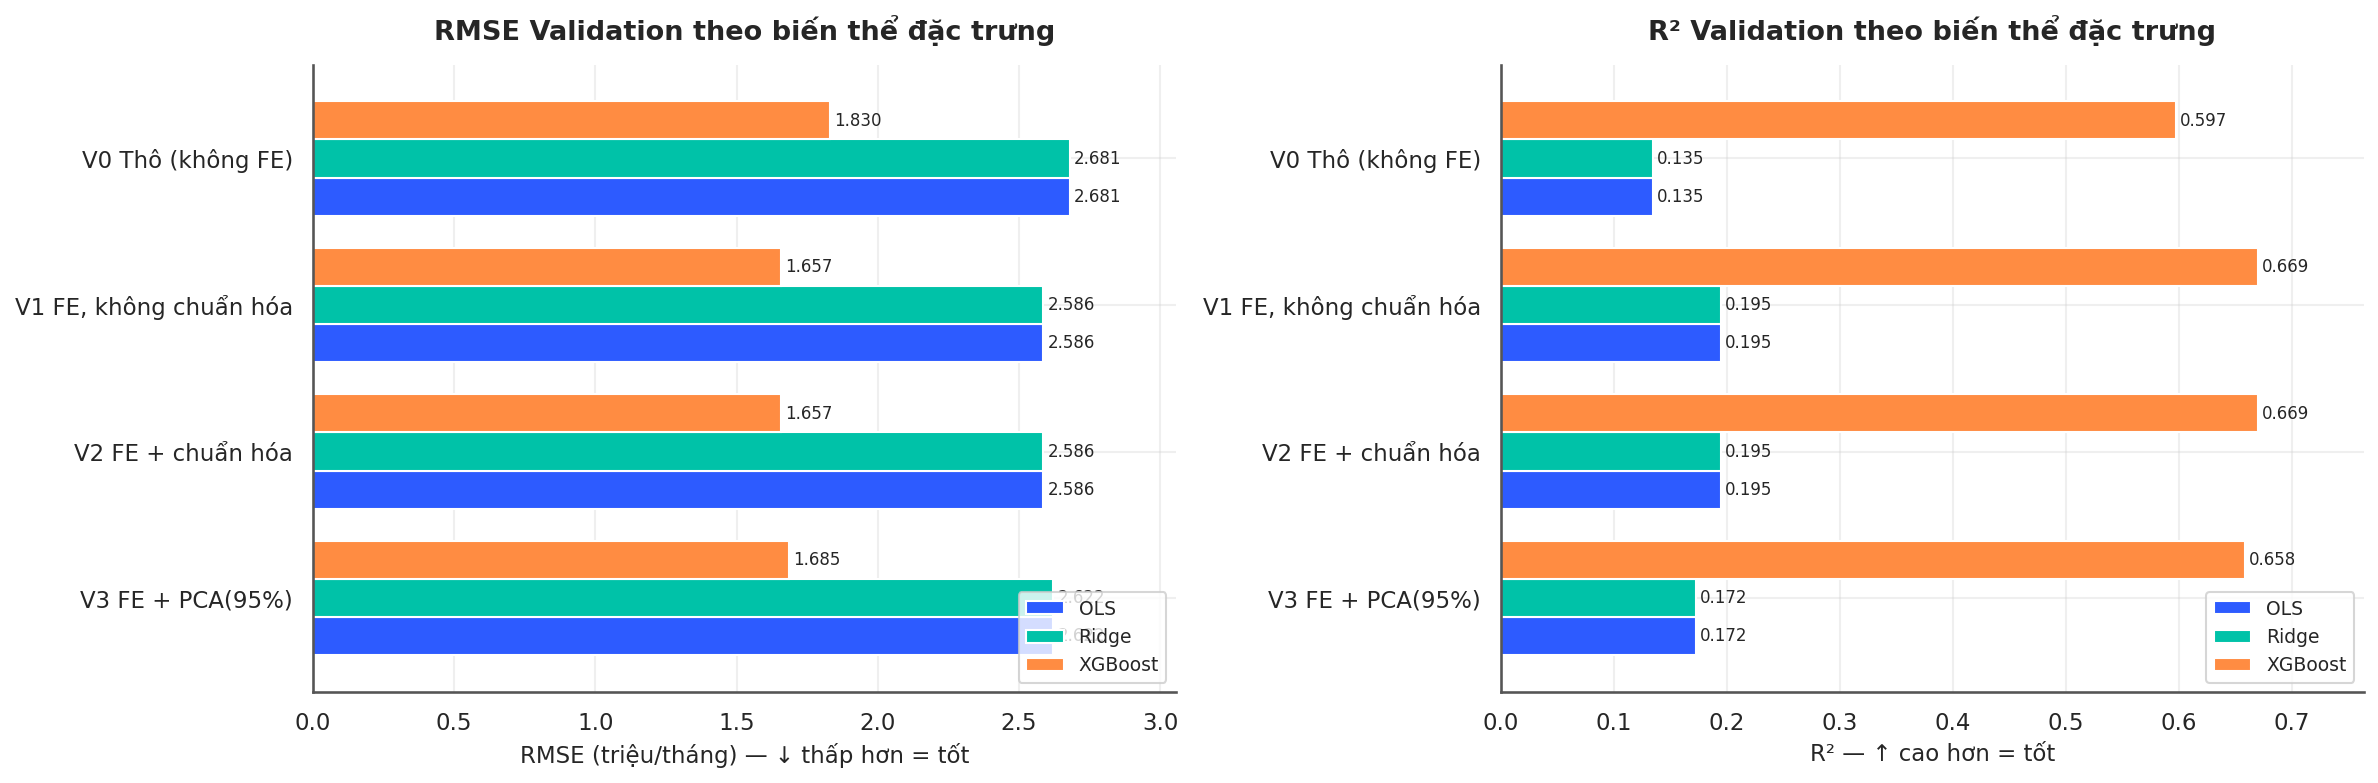
\includegraphics[width=0.90\textwidth]{abl_04_fe_pca}
  \caption{Thực nghiệm A — RMSE và R\textsuperscript{2} theo 4 biến thể đặc trưng.
           FE cải thiện RMSE 3.5\% (tuyến tính) đến 9.4\% (XGBoost) so với dữ liệu thô;
           thêm PCA lại làm tệ hơn 1.4--1.7\%}
  \label{fig:abl_fe}
\end{figure}

\textbf{Kết luận và quyết định:}
{\sloppy
\begin{itemize}[leftmargin=*, itemsep=2pt]
  \item \textbf{Dùng FE (V2):} tách \texttt{city}\slash\texttt{district} từ \texttt{full\_address}
        giảm RMSE \textbf{3.5\% (tuyến tính) đến 9.4\% (XGBoost)} — nguồn cải thiện là
        \textit{mở khóa tín hiệu khu vực} ẩn trong chuỗi địa chỉ (đúng trọng tâm đề tài
        ``theo khu vực'').
  \item \textbf{Không dùng PCA:} $\approx$80 chiều sau One-Hot chưa đủ cao để PCA phát huy;
        nén về $\approx$95\% phương sai loại bỏ mất tín hiệu quận/huyện quan trọng → RMSE tệ hơn.
  \item \textbf{Giữ chuẩn hóa:} không đổi kết quả với OLS/XGBoost
        (bất biến co giãn tuyến tính), nhưng cần thiết cho Ridge/LASSO và PCA.
\end{itemize}
}

\fbox{\textbf{Quyết định A:} Pipeline dứt khoát dùng \textbf{FE + chuẩn hóa Z-score (V2)}.}

% ─────────────────────────────────────────────────────────────────
\subsection[Thực nghiệm B — Biến mục tiêu: price gốc vs. log1p(price)]{Thực nghiệm B — Biến mục tiêu: \texttt{price} gốc vs.\ $\log(1+\text{price})$}
\label{subsec:abl_log}

\textbf{Câu hỏi:} Log-transform biến mục tiêu có thực sự tăng hiệu năng, hay làm mô hình
``underweight'' phân khúc giá cao?
(Giá cao đều có nguyên nhân thực: vị trí trung tâm, đầy đủ tiện ích.)

\textbf{Thiết kế:} ngoài MAE/RMSE/R\textsuperscript{2} toàn cục, đo riêng
\textbf{bias phân khúc giá cao} ($\geq$10 triệu/tháng, 8.3\% Validation):
$\text{bias} = \overline{\hat{y} - y}$; âm nhiều = dự đoán hụt hệ thống.

\begin{table}[H]
  \centering
  \caption{Đối sánh mục tiêu — \texttt{price} gốc vs.\ $\log1p(\text{price})$}
  \label{tab:abl_log}
  \small
  \begin{tabular}{@{}l l r r r r@{}}
    \toprule
    \textbf{Mô hình} & \textbf{Mục tiêu} &
    \textbf{MAE} & \textbf{RMSE} & \textbf{R\textsuperscript{2}} &
    \textbf{Bias giá cao ($\geq$10tr)} \\
    \midrule
    OLS & \textbf{price gốc}  & 1.963 & \textbf{2.586} & \textbf{0.195} & $-5.61$ triệu \\
    OLS & log1p(price) & \textbf{1.882} & 2.636 & 0.164 & $-6.31$ triệu \\
    \addlinespace
    XGBoost & \textbf{price gốc}  & 0.990 & \textbf{1.657} & \textbf{0.669} & $-2.34$ triệu \\
    XGBoost & log1p(price) & \textbf{0.975} & 1.694 & 0.655 & $-2.78$ triệu \\
    \bottomrule
  \end{tabular}
\end{table}

\begin{figure}[H]
  \centering
  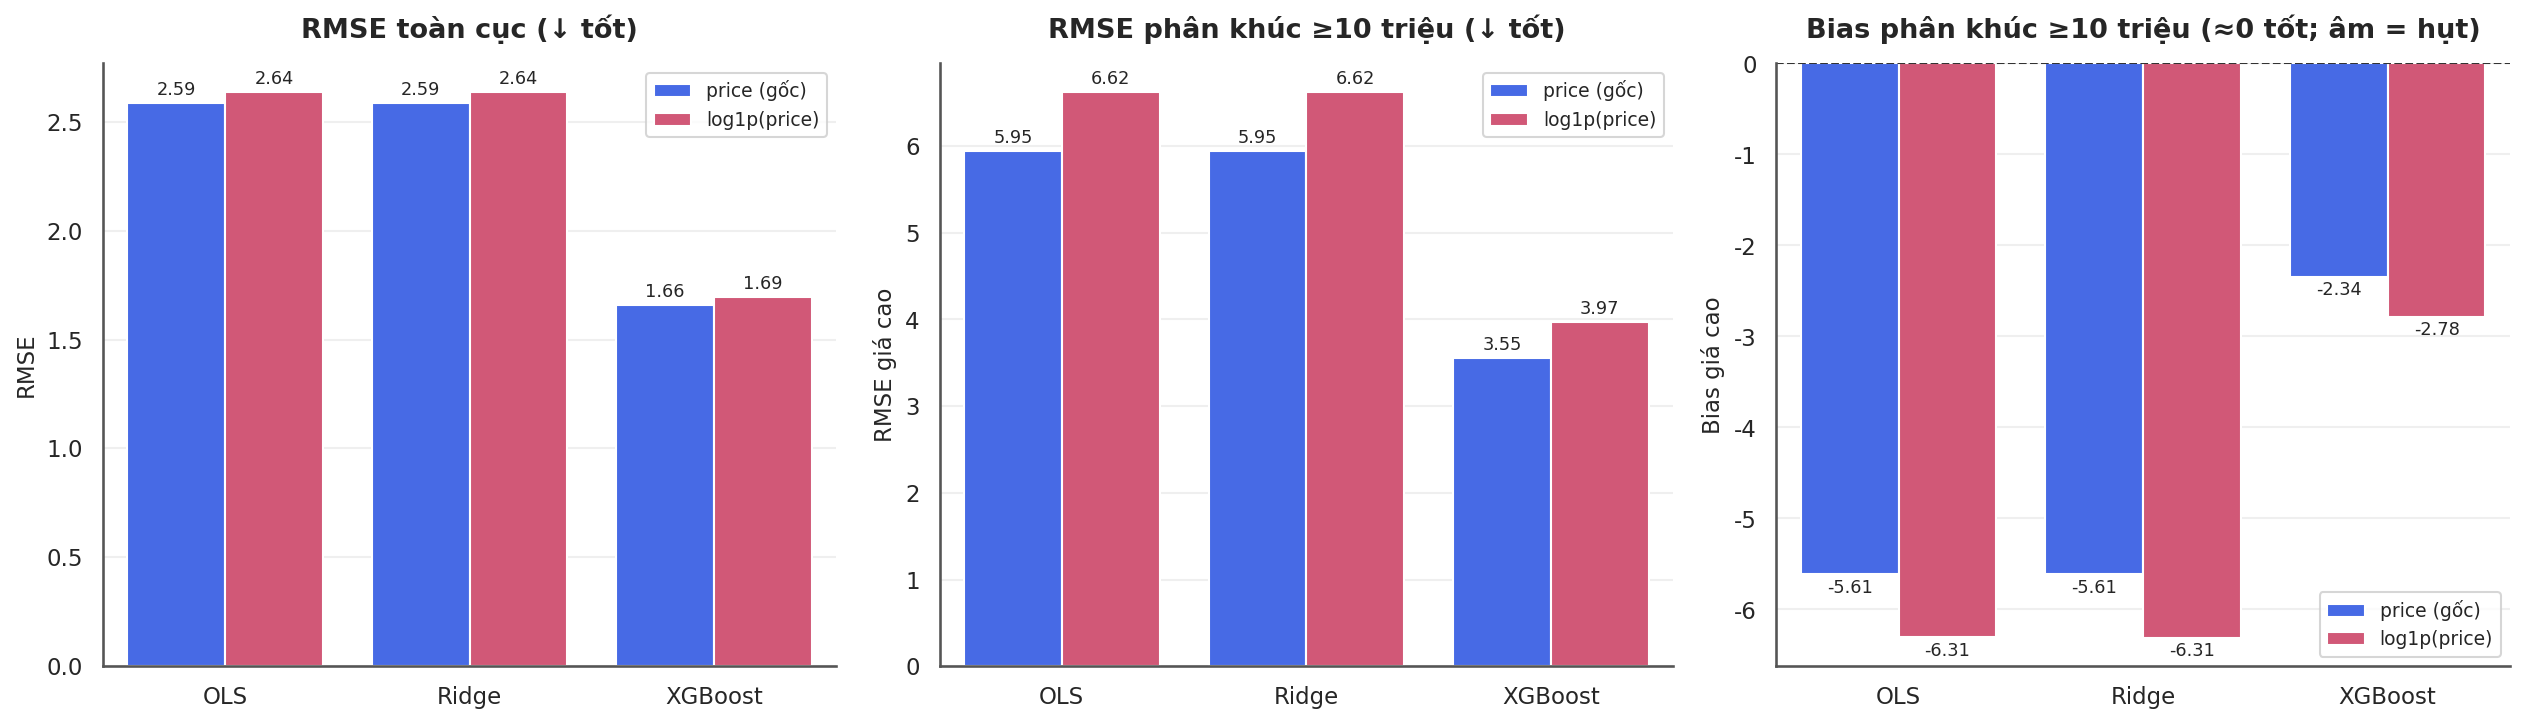
\includegraphics[width=0.90\textwidth]{abl_05_log_target}
  \caption{Thực nghiệm B — RMSE toàn cục (trái), RMSE phân khúc giá cao (giữa),
           Bias giá cao (phải).
           Log chỉ giảm MAE nhẹ; RMSE và bias phân khúc giá cao đều tệ hơn}
  \label{fig:abl_log}
\end{figure}

\textbf{Kết luận và quyết định:}
\begin{itemize}[leftmargin=*, itemsep=2pt]
  \item Log cải thiện MAE $\approx$1.6--4.1\%, nhưng \textbf{RMSE tăng 1.9--2.2\%} và R\textsuperscript{2}
        giảm — không cải thiện theo tiêu chí chọn mô hình chính (RMSE).
  \item \textbf{Bias phân khúc giá cao âm sâu hơn:}
        OLS $-5.61 \to -6.31$ triệu; XGBoost $-2.34 \to -2.78$ triệu.
        Đúng hiện tượng \textit{underweight}: log nén phân khúc giá cao, làm mô hình
        đánh giá thấp các căn hộ đắt dù chúng có nguyên nhân giá thực sự.
  \item Gợi ý log từ phân tích phân phối (EDA) \textbf{bị thực nghiệm bác bỏ}.
\end{itemize}

\fbox{\textbf{Quyết định B:} Cả 5 mô hình huấn luyện trực tiếp trên \textbf{\texttt{price} gốc}.}

% ─────────────────────────────────────────────────────────────────
\subsection{Thực nghiệm C — Tác động của ngoại lệ trong tập huấn luyện}
\label{subsec:abl_outlier}

\textbf{Câu hỏi:} Nếu giữ lại ngoại lệ (giá tới 10.000 triệu $\approx$ 10 tỷ/tháng,
diện tích tới 1.000 m\textsuperscript{2}), hiệu năng trên vùng giá mục tiêu thay đổi thế nào?

\textbf{Thiết kế:} hai mô hình XGBoost hoàn toàn giống nhau, chỉ khác tập Train
(có / không có 6.8\% ngoại lệ);
chấm trên cùng tập Validation vùng mục tiêu (\texttt{price}$\leq$17, \texttt{area}$\leq$180).

\begin{table}[H]
  \centering
  \caption{XGBoost — cùng Validation vùng mục tiêu, chỉ khác tập Train}
  \label{tab:abl_out}
  \begin{tabular}{@{}l c c@{}}
    \toprule
    \textbf{Tập Train} & \textbf{RMSE Validation} & \textbf{So với pipeline chính} \\
    \midrule
    Có ngoại lệ (6.8\% outlier) & 9.747 & $+490\%$ \\
    \textbf{Đã lọc ngoại lệ (pipeline chính)} & \textbf{1.652} & — \\
    \bottomrule
  \end{tabular}
\end{table}

\begin{figure}[H]
  \centering
  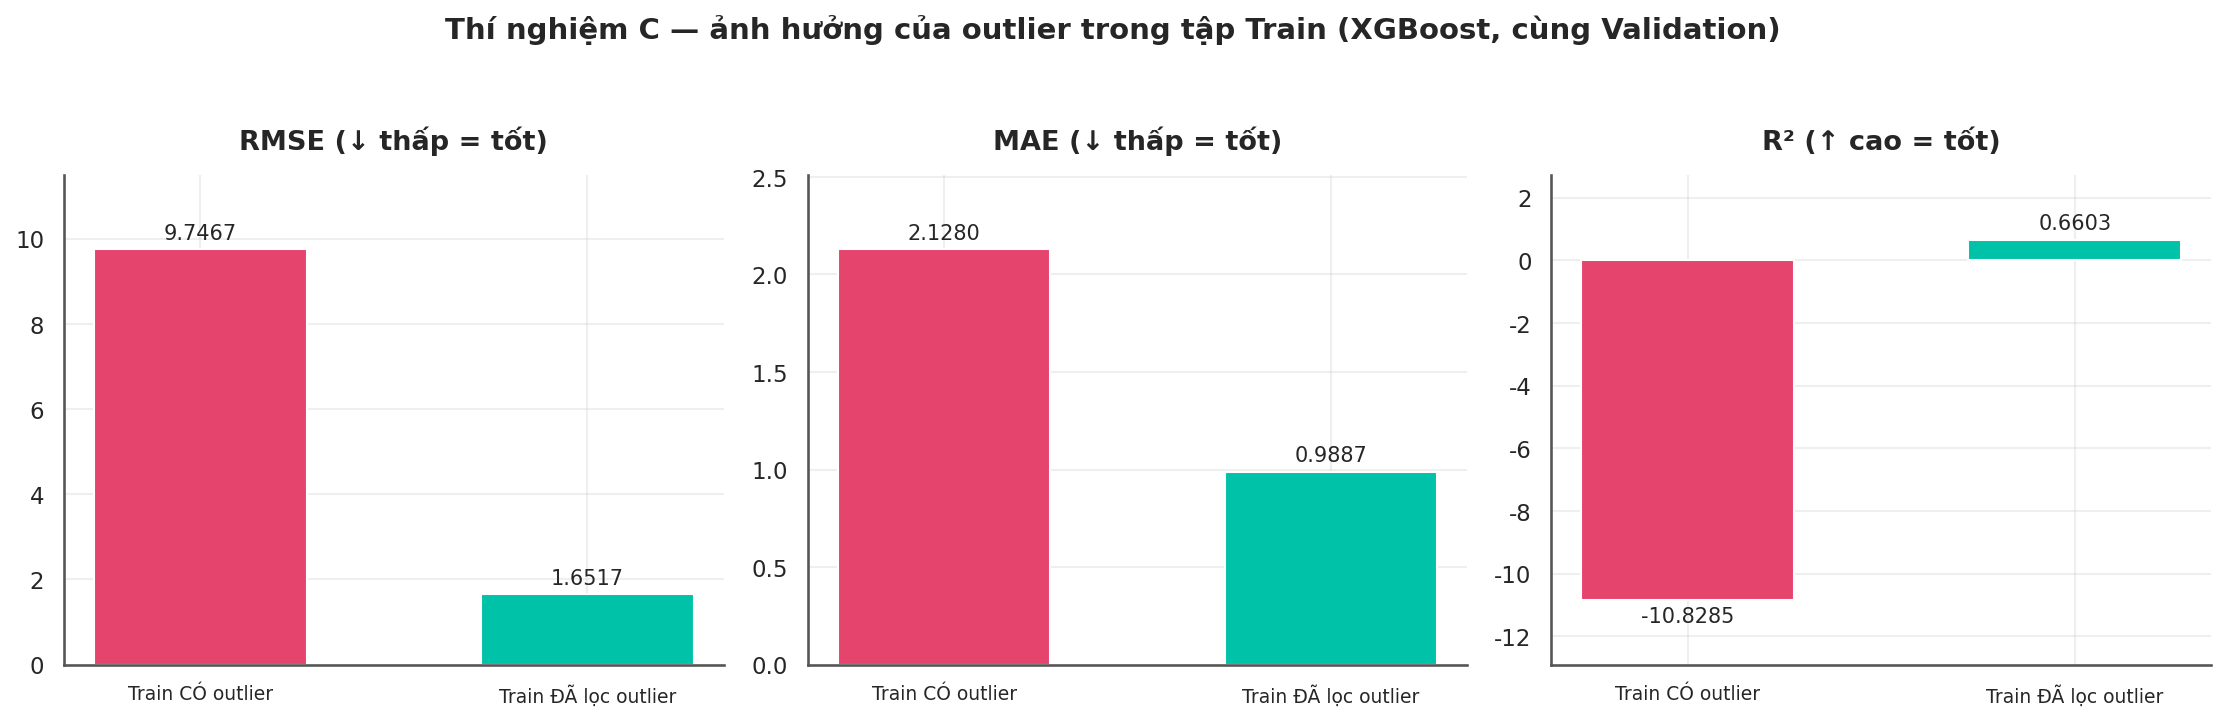
\includegraphics[width=0.90\textwidth]{abl_06_outliers}
  \caption{Thực nghiệm C — RMSE của XGBoost có / không outlier trong Train.
           Giữ outlier làm RMSE xấu hơn $\approx$5.9 lần trên vùng giá mục tiêu}
  \label{fig:abl_out}
\end{figure}

\textbf{Kết luận và quyết định:}
Giữ lại bản ghi giá hàng tỷ/tháng kéo lệch hàm mất mát bình phương —
mô hình phân bổ năng lực học cho vùng giá không bao giờ xuất hiện trong thực tế.
Lọc ngoại lệ giảm RMSE \textbf{83.1\%} trên vùng mục tiêu.

\fbox{\textbf{Quyết định C:} \textbf{Lọc outlier} (\texttt{price}$\leq$17, \texttt{area}$\leq$180) trước khi huấn luyện.}

% ─────────────────────────────────────────────────────────────────
\subsection{Tổng hợp quyết định pipeline}
\label{subsec:pipeline_summary}

Sau 3 thực nghiệm đối sánh, \textbf{pipeline dứt khoát} được xác định:

\begin{table}[H]
  \centering
  \caption{Tổng hợp 3 quyết định thiết kế pipeline — có kiểm chứng thực nghiệm}
  \label{tab:pipeline}
  \begin{tabularx}{\textwidth}{@{}l X l@{}}
    \toprule
    \textbf{Quyết định} & \textbf{Lý do (từ số liệu)} & \textbf{Thực nghiệm} \\
    \midrule
    FE: tách \texttt{city}/\texttt{district} & Giảm RMSE 3.5--9.4\%; PCA không giúp ích & A \\
    Mục tiêu: \texttt{price} gốc & Log tăng RMSE + underweight giá cao & B \\
    Lọc outlier: price$\leq$17, area$\leq$180 & Không lọc làm RMSE $\times$5.9 & C \\
    Mask MNAR + bỏ \texttt{n\_features} + ràng buộc đơn điệu &
      7/12 cờ tiện ích chế tác; hiệu ứng tiện ích âm phi lý & D (Mục~\ref{subsec:audit}) \\
    \bottomrule
  \end{tabularx}
\end{table}

\textbf{Kết quả ở Mục~\ref{subsec:main_results} dưới đây được tính trên pipeline sau
quyết định A--C} (so sánh họ mô hình và chọn mô hình triển khai); quyết định D đến từ
kiểm toán \textit{sau} bước này và chỉ áp dụng cho mô hình triển khai
(Mục~\ref{subsec:audit}).

% ─────────────────────────────────────────────────────────────────
\subsection{Kết quả chính: 10-fold CV và đánh giá Test}
\label{subsec:main_results}

5 mô hình được huấn luyện và đánh giá với \textbf{pipeline đã được xác nhận} ở Mục~\ref{subsec:pipeline_summary}:
dùng FE (city/district), mục tiêu \texttt{price} gốc, dữ liệu đã lọc ngoại lệ.

\begin{table}[H]
  \centering
  \caption{So sánh 5 mô hình — 10-fold CV (Train+Val) và đánh giá Test 1 lần duy nhất.
           $\star$ = mô hình triển khai.}
  \label{tab:model_compare}
  \begin{tabular}{@{}l r@{$\;\pm\;$}l r r r r@{}}
    \toprule
    \textbf{Mô hình} &
    \multicolumn{2}{c}{\textbf{CV RMSE}} &
    \textbf{CV R\textsuperscript{2}} &
    \textbf{Test MAE} & \textbf{Test RMSE} & \textbf{Test R\textsuperscript{2}} \\
    \midrule
    OLS           & 2.582 & 0.018 & 0.193 & 1.958 & 2.586 & 0.190 \\
    Ridge         & 2.582 & 0.018 & 0.193 & 1.958 & 2.586 & 0.190 \\
    LASSO         & 2.587 & 0.019 & 0.190 & 1.961 & 2.589 & 0.188 \\
    Random Forest & \textbf{1.657} & 0.012 & \textbf{0.668} & \textbf{1.002} & \textbf{1.666} & \textbf{0.664} \\
    \midrule
    \textbf{XGBoost} $\star$
      & 1.881 & 0.008 & 0.572 & 1.257 & 1.895 & 0.565 \\
    \bottomrule
  \end{tabular}
\end{table}

\begin{figure}[H]
  \centering
  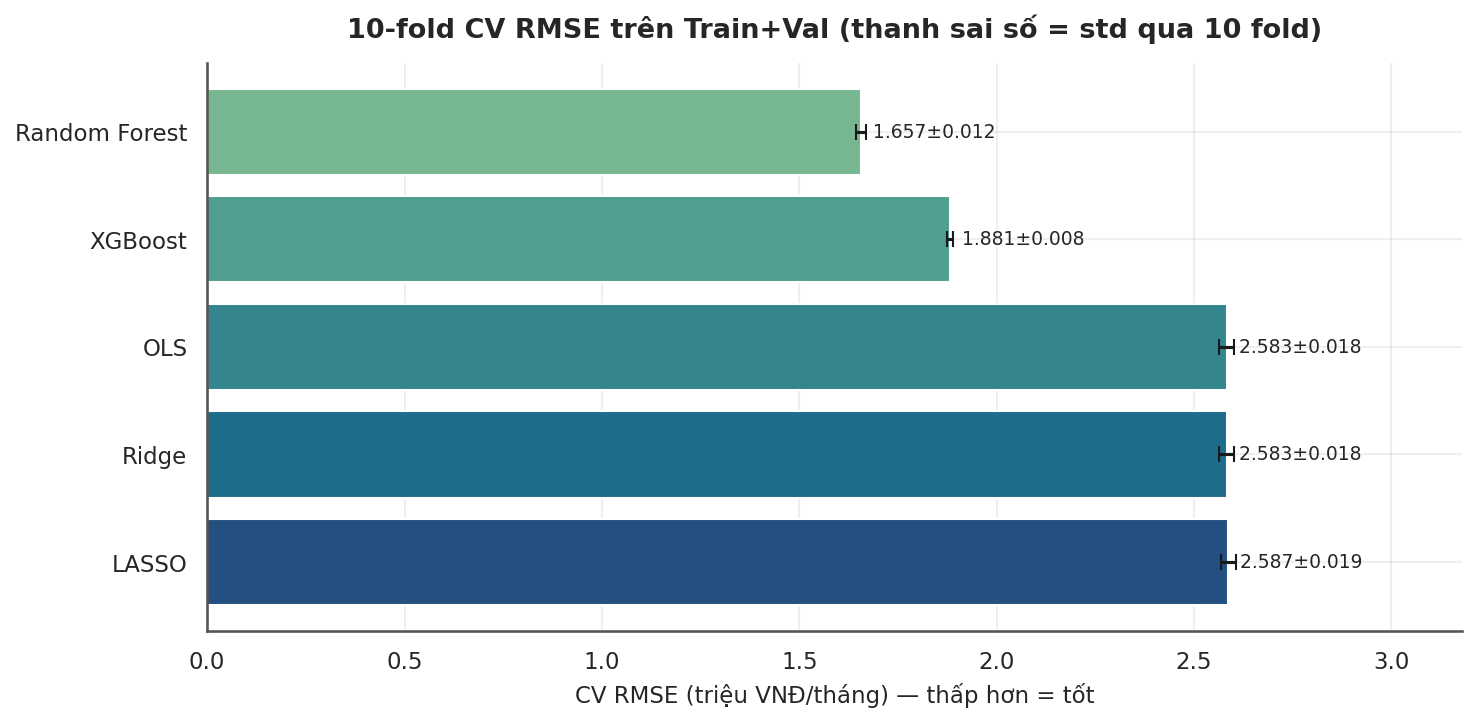
\includegraphics[width=0.86\textwidth]{eval_01_cv_rmse_comparison}
  \caption{CV RMSE của 5 mô hình (mean $\pm$ std, 10 fold) —
           mô hình cây vượt trội (RF $\approx$1.66, XGBoost $\approx$1.88 vs.\ $\approx$2.58 của
           tuyến tính); std nhỏ xác nhận ổn định qua các cách chia}
  \label{fig:cv_compare}
\end{figure}

\begin{figure}[H]
  \centering
  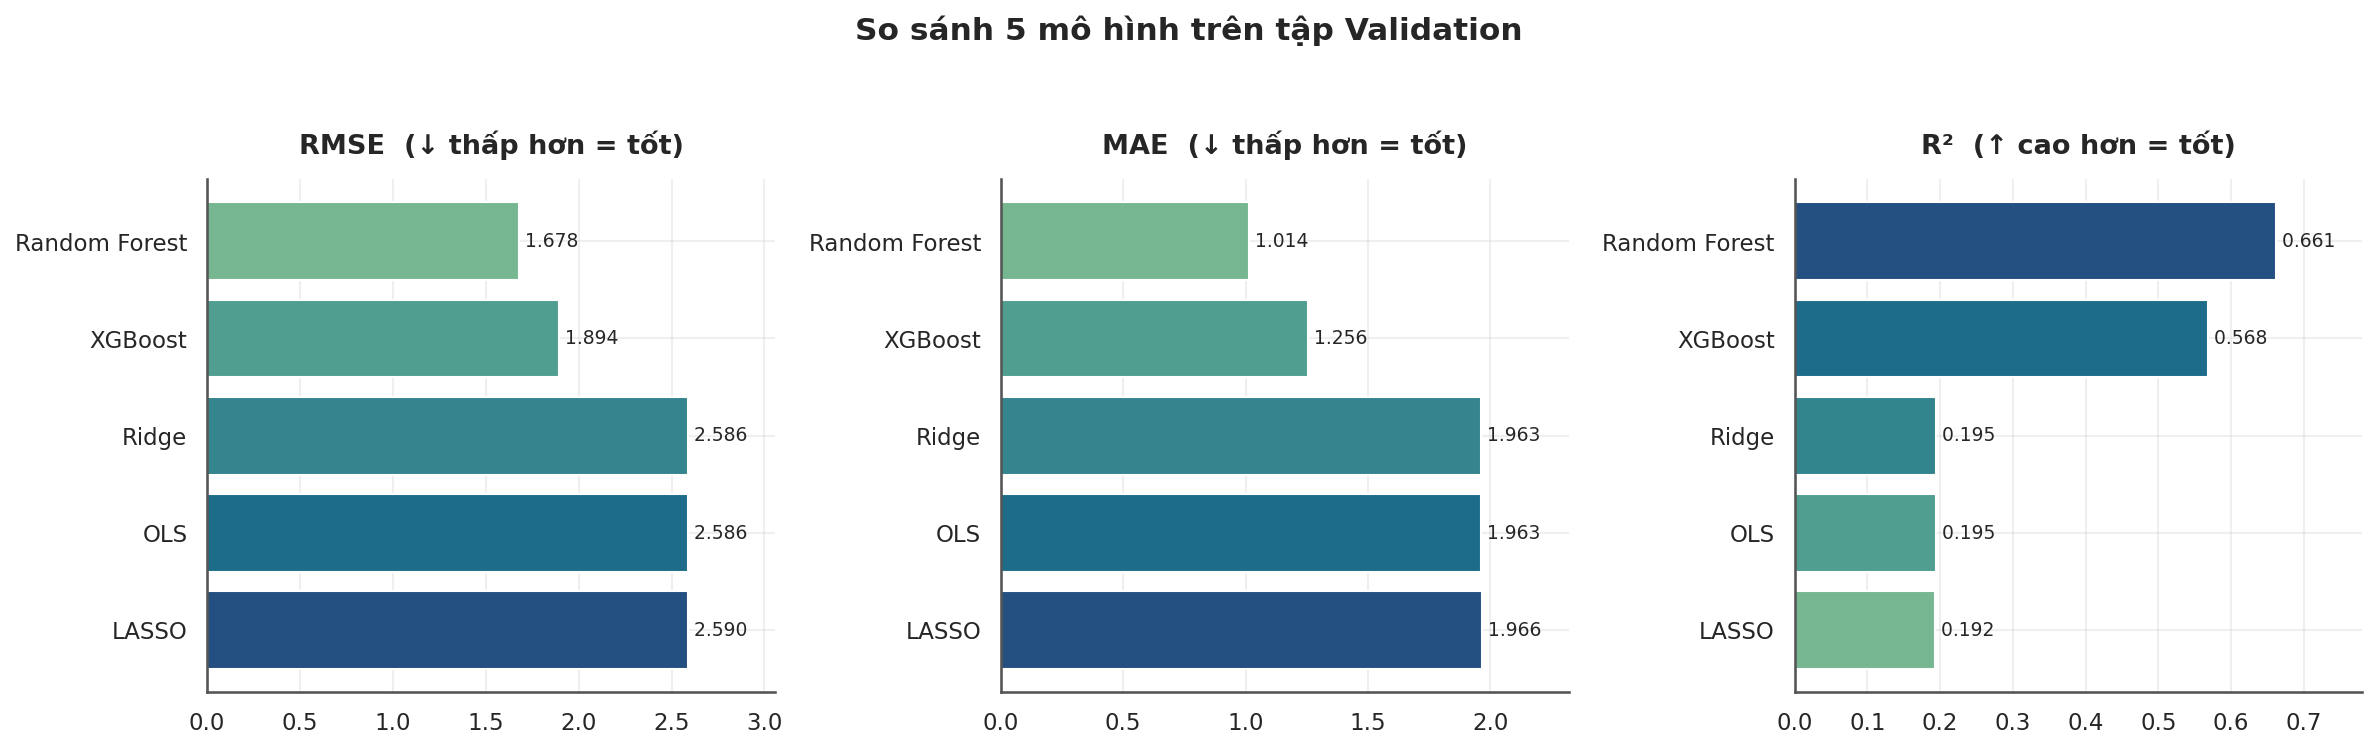
\includegraphics[width=0.86\textwidth]{model_01_model_comparison_val}
  \caption{So sánh RMSE, MAE và R\textsuperscript{2} trên tập Validation — hai mô hình cây
           cách xa tuyến tính; Random Forest nhỉnh hơn XGBoost (XGBoost có ràng buộc đơn điệu
           nên đánh đổi một phần chỉ số lấy hành vi đúng — Mục~\ref{subsec:audit})}
  \label{fig:val_compare}
\end{figure}

\textbf{Phân tích kết quả:}
\begin{itemize}[leftmargin=*, itemsep=3pt]
  \item Mô hình cây \textbf{vượt trội rõ rệt} so với tuyến tính
        (Test R\textsuperscript{2}: $\approx$0.57--0.66 vs.\ $\approx$0.19),
        xác nhận quan hệ phi tuyến và tương tác khu vực $\times$ diện tích
        được gợi ý từ PCA ở Mục~\ref{subsec:clustering}.
  \item CV RMSE $\approx$ Test RMSE, std nhỏ $\Rightarrow$ mô hình \textbf{không overfit},
        khái quát hóa tốt.
  \item \textbf{Chính xác nhất là Random Forest} (Test R\textsuperscript{2} = 0.664), nhưng
        \textbf{mô hình triển khai là XGBoost} (Test R\textsuperscript{2} = 0.565) vì hai lý do
        \textit{vượt trên chỉ số thô}:
        \begin{enumerate}[leftmargin=1.2em, itemsep=1pt, topsep=2pt]
          \item \textbf{Hành vi đúng cho app:} XGBoost mang \textbf{ràng buộc đơn điệu} đảm bảo
                tick thêm tiện ích không làm giảm giá (Mục~\ref{subsec:audit}); Random Forest ở
                đây chạy \textit{không ràng buộc}, nên một phần độ chính xác của nó đến từ tự do
                khai thác tương quan hành-vi-đăng-tin phi nhân quả — sai với người dùng app.
          \item \textbf{Triển khai được:} XGBoost $\approx$0.86 MB so với Random Forest $\approx$5.6 MB
                ($n=200$ cây), nạp/suy luận nhanh hơn trong app, lại có early stopping.
        \end{enumerate}
        Khoảng cách 0.664 vs.\ 0.565 chính là \textbf{cái giá có chủ đích} của việc từ chối
        tương quan phi nhân quả (phân tích kỹ ở Mục~\ref{subsec:audit}).
\end{itemize}

% ─────────────────────────────────────────────────────────────────
\subsection{Biểu đồ chẩn đoán mô hình triển khai (XGBoost)}
\label{subsec:diagnostics}

\begin{figure}[H]
  \centering
  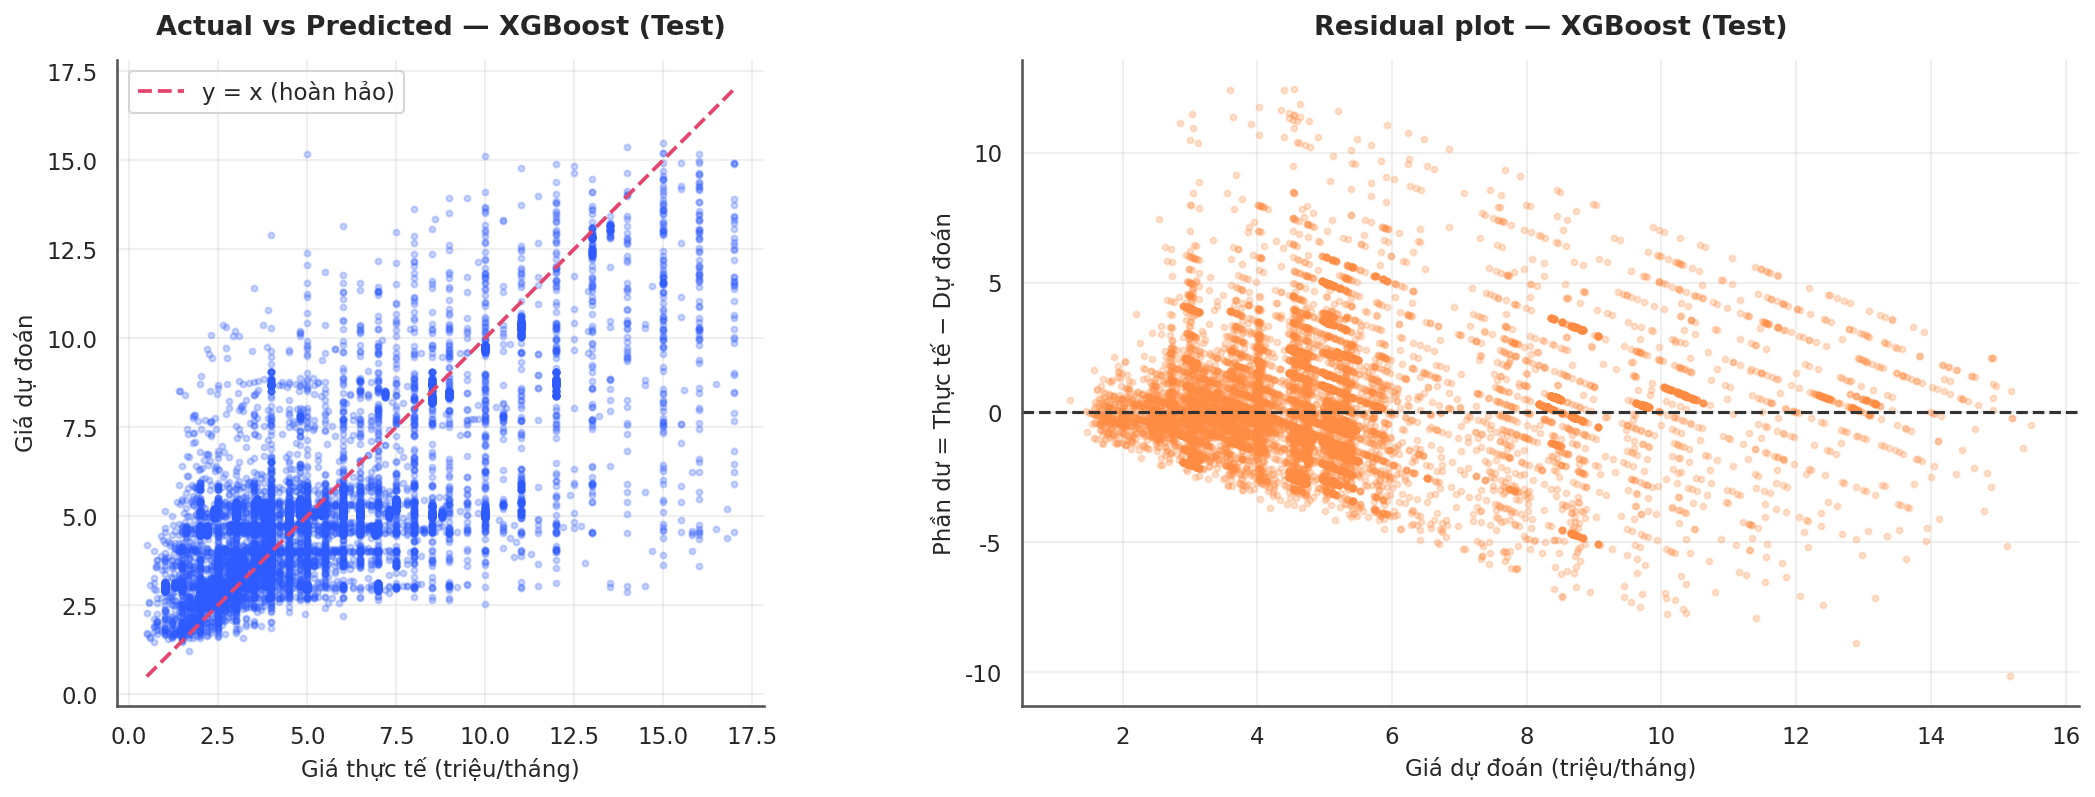
\includegraphics[width=0.86\textwidth]{eval_02_test_actual_vs_pred}
  \caption{Test — Actual vs Predicted (trái) và Residual vs Predicted (phải).
           Điểm bám sát đường $y=x$; phần dư phân tán quanh 0 (mean $\approx$0)
           $\Rightarrow$ không thiên lệch hệ thống}
  \label{fig:test_pred}
\end{figure}

\begin{figure}[H]
  \centering
  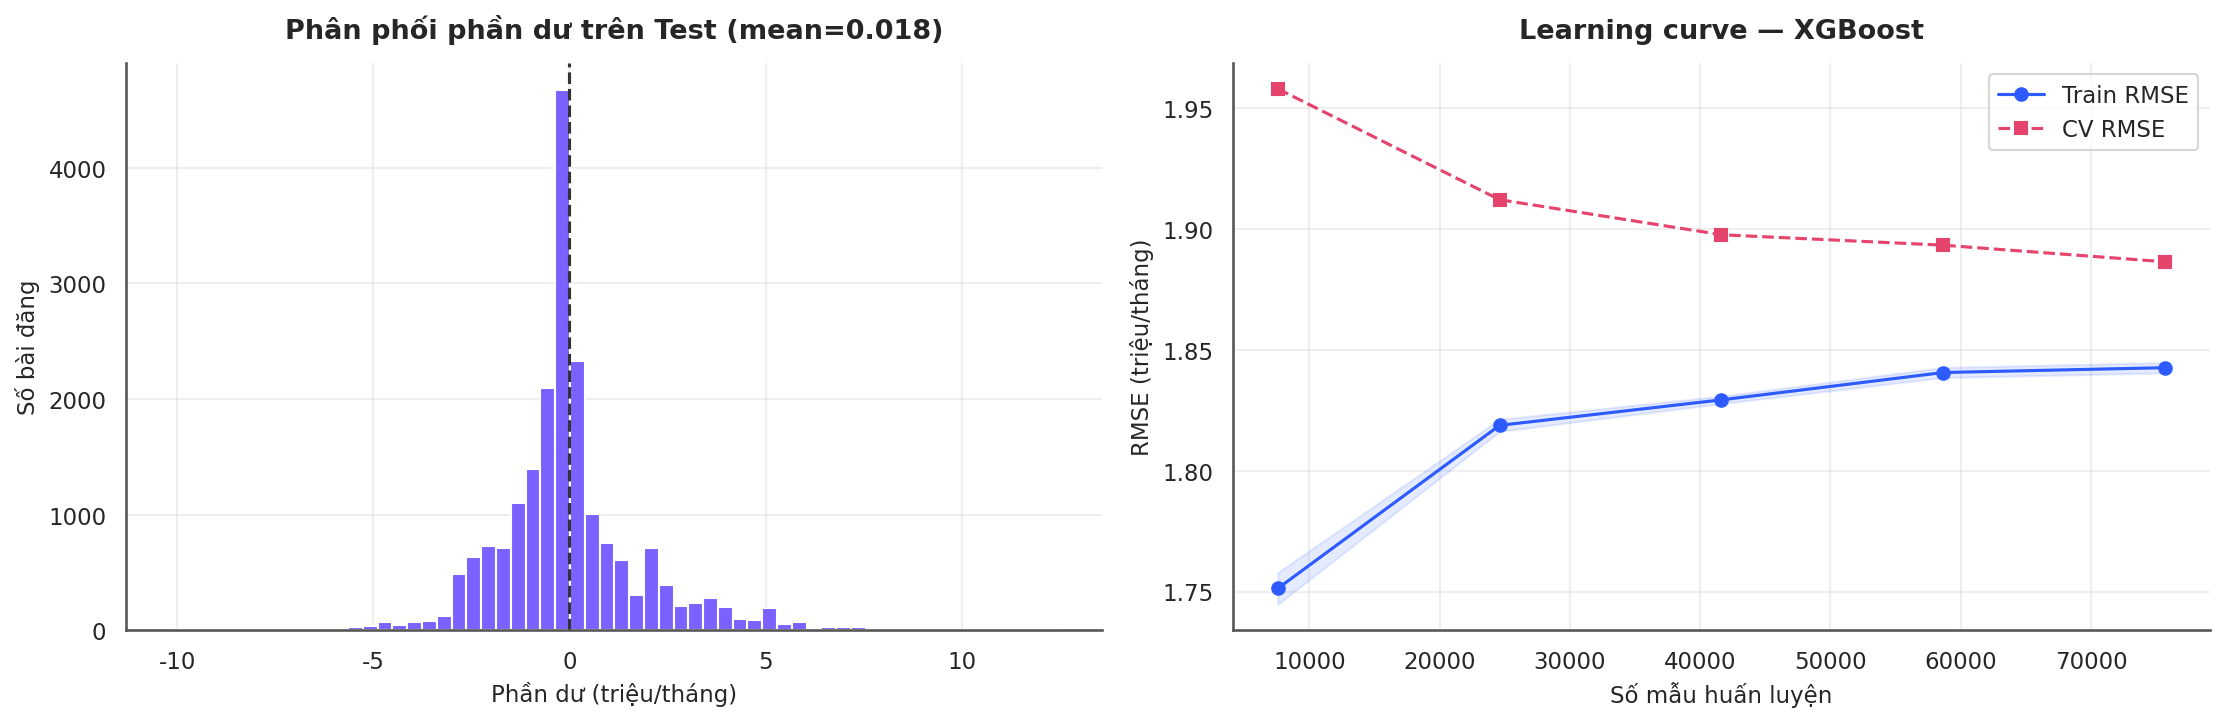
\includegraphics[width=0.86\textwidth]{eval_03_residual_learning_curve}
  \caption{Phân phối phần dư (trái) và Learning curve (phải).
           Train RMSE và CV RMSE hội tụ khi tăng dữ liệu $\Rightarrow$ không overfit nặng;
           khoảng cách còn lại là \textit{bias} — cần đặc trưng mới (GPS, NLP mô tả)}
  \label{fig:lc}
\end{figure}

\begin{figure}[H]
  \centering
  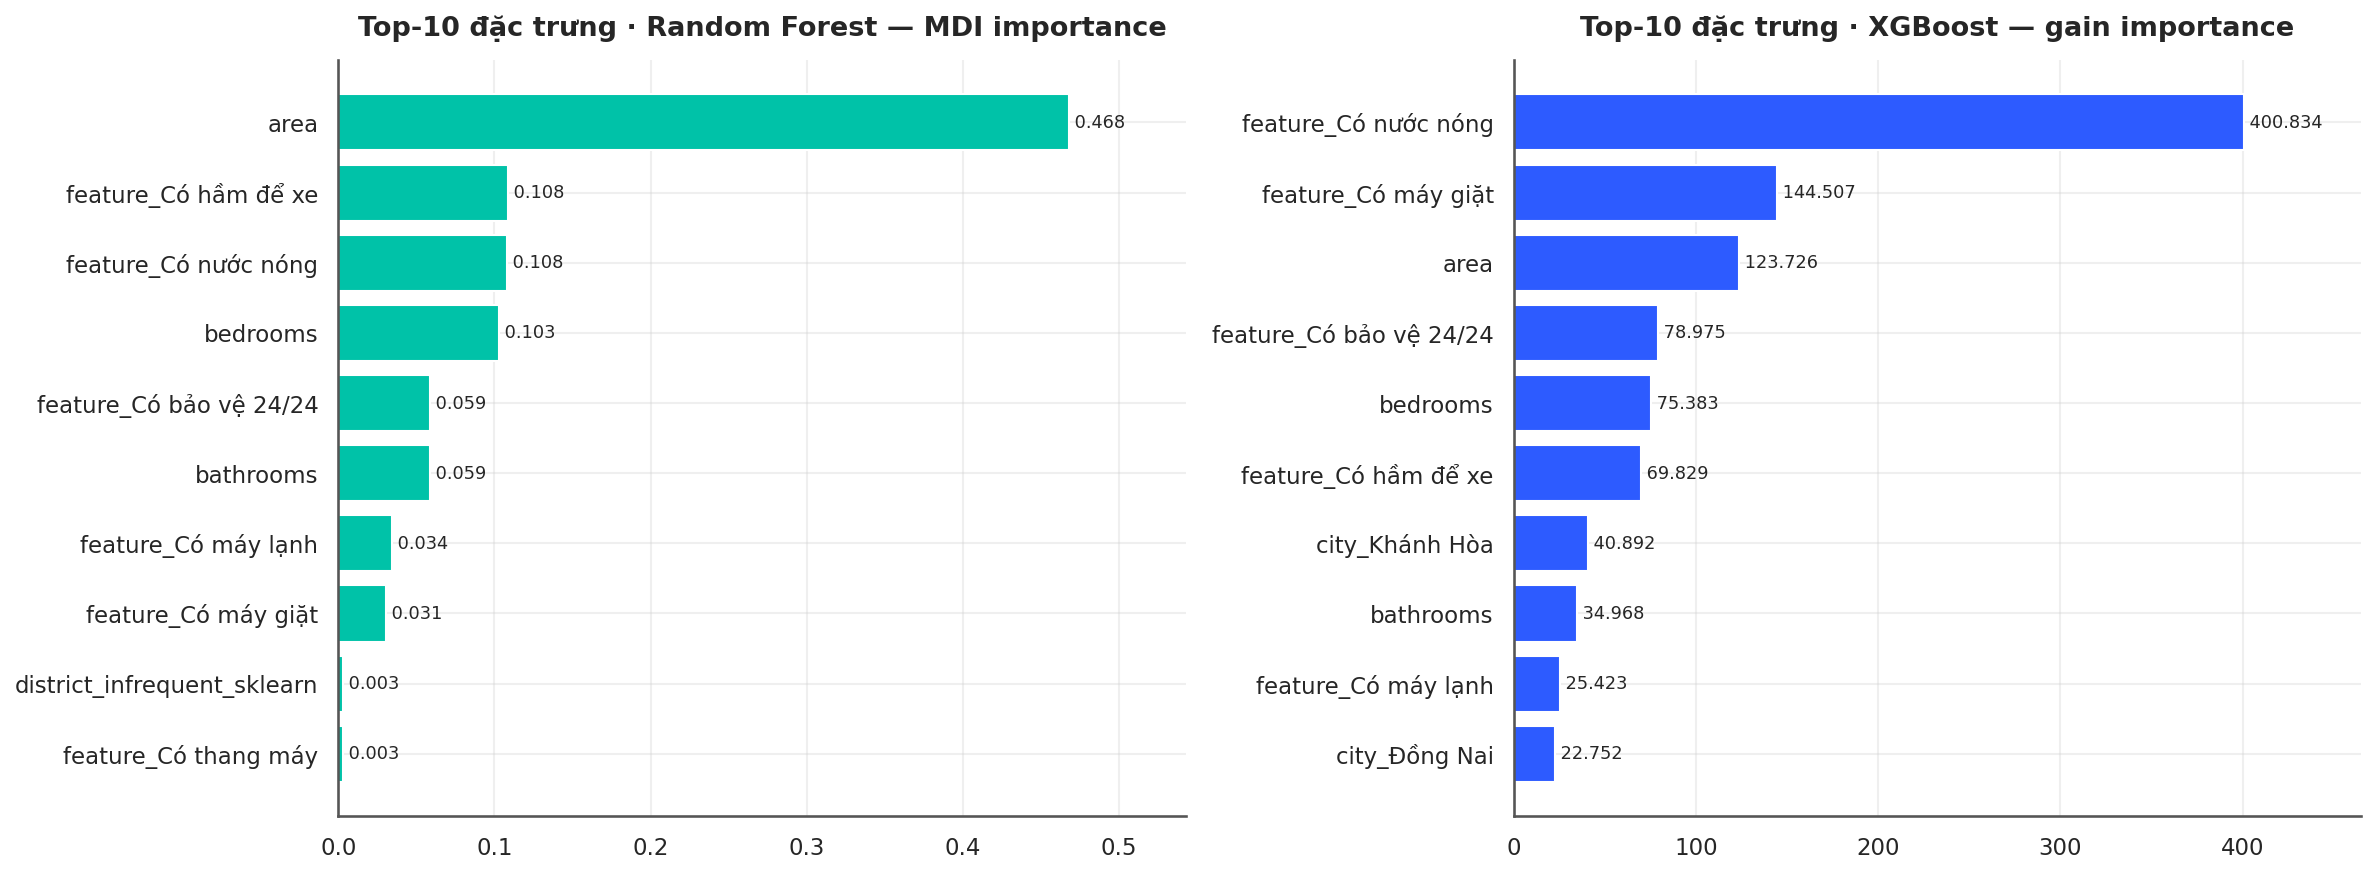
\includegraphics[width=0.84\textwidth]{model_02_feature_importance}
  \caption{Feature Importance — RF (MDI, trái) và XGBoost (gain, phải).
           Sau khi loại \texttt{source}, đặc trưng dẫn đầu là \texttt{area} và
           tiện ích/khu vực — đúng yếu tố định giá thực tế,
           xác nhận giá trị của FE (Thực nghiệm A)}
  \label{fig:importance}
\end{figure}

% ─────────────────────────────────────────────────────────────────
\subsection{Thực nghiệm D — Kiểm toán sau triển khai: cờ tiện ích chế tác
            (MNAR) và ràng buộc đơn điệu}
\label{subsec:audit}

\subsubsection*{Hiện tượng kích hoạt: kiểm thử hành vi trên app demo}

Chỉ số tổng hợp (RMSE/R\textsuperscript{2}) không nói hết về một mô hình.
Khi kiểm thử app demo với input điển hình (25 m\textsuperscript{2}, 1 phòng ngủ,
1 phòng tắm, Hà Nội), việc \textbf{tick ``Có máy lạnh'' làm giá dự báo GIẢM 0.34
triệu/tháng} — phi lý về kinh tế học. Phân rã hiệu ứng cho thấy ngoài máy lạnh
($-0.34$), ba tiện ích khác cũng mang hiệu ứng âm (máy giặt $-0.42$, nước nóng $-0.27$,
hầm để xe $-0.17$), và đường ``tick dần 12 tiện ích''
\textbf{không đơn điệu} (vi phạm 7 lần).

\subsubsection*{Điều tra nguyên nhân: dấu vân tay nguồn}

Phân tích phân tầng chỉ ra cơ chế: nguồn \texttt{nhatot} là phân khúc đắt
(trung vị \textbf{9.0} triệu so với $\approx$4.0 triệu của các nguồn khác) nhưng tỷ lệ
bật cờ tiện ích thấp bất thường (máy lạnh 22\% so với 67--75\% nơi khác; máy giặt 11\%;
nước nóng 6\%). Hệ quả là nhóm ``máy lạnh = 0'' chứa 18.7\% tin \texttt{nhatot}, còn nhóm
``máy lạnh = 1'' chỉ 2.4\% — vì \texttt{source} đã bị loại (đúng đắn, Mục~\ref{subsec:simpson}),
mô hình dùng \textit{pattern cờ tiện ích như dấu vân tay nguồn}: ``không tick máy lạnh
$\Rightarrow$ giống tin nhatot $\Rightarrow$ đắt''. Trong khi đó, hiệu ứng thật của máy lạnh
\textit{trong từng nguồn} và trong đúng phân khúc app dự báo (Hà Nội, 20--30 m\textsuperscript{2})
là $\approx 0$ đến $+0.2$ triệu.

\subsubsection*{Kiểm toán nguồn gốc dữ liệu: 7/12 cờ bị chế tác}

Truy ngược về dữ liệu thô của từng nguồn (đối chiếu tỷ lệ bật cờ
raw $\leftrightarrow$ sau hợp nhất) phát hiện vấn đề nghiêm trọng hơn:

\begin{table}[H]
  \centering
  \caption{Kiểm toán nguồn gốc 12 cờ tiện ích: cờ có cột gốc thật theo nguồn}
  \label{tab:audit_flags}
  \small
  \begin{tabularx}{\textwidth}{@{}L{4.6cm} C{2.2cm} X@{}}
    \toprule
    \textbf{Nguồn} & \textbf{Số cờ thật} & \textbf{Ghi chú} \\
    \midrule
    chothuephongtro, nhatot,\newline facebook, github\_housing & 5/12 &
      máy lạnh, máy giặt, nước nóng, bảo vệ 24/24, hầm để xe
      (tỷ lệ raw $\leftrightarrow$ hợp nhất khớp tới $\approx$1\%) \\
    lozido & 10/12 & thêm gác, kệ bếp, thang máy, không chung chủ, giờ giấc \\
    phongtro123 & 11/12 & thiếu duy nhất nước nóng \\
    chothuenhadattoanvn,\newline github\_hcm/hn/dn ($\approx$16.6\% dữ liệu) & \textbf{0/12} &
      dữ liệu thô không có cột tiện ích nào \\
    \bottomrule
  \end{tabularx}
\end{table}

Bảy cờ còn lại (tủ lạnh, nội thất, gác, kệ bếp, thang máy, không chung chủ, giờ giấc)
chỉ tồn tại thật ở \texttt{phongtro123} + \texttt{lozido} ($\approx$3\% dữ liệu);
với các nguồn khác chúng được \textbf{điền ngẫu nhiên ở bước tích hợp} —
bằng chứng thống kê: tương quan với giá \textit{trong từng nguồn} của các ô chế tác
$\leq 0.013$ (bằng 0 tuyệt đối, đặc trưng của biến ngẫu nhiên độc lập).
Đây cũng chính là lời giải cho các tương quan ``chết'' ở Bảng~\ref{tab:simpson}.

\subsubsection*{Bản vá ba lớp và kết quả}

\begin{enumerate}[leftmargin=*, itemsep=2pt]
  \item \textbf{Mask MNAR:} ô (nguồn, cờ) chế tác $\to$ NaN — ``không khai báo''
        $\neq$ ``không có''. XGBoost xử lý NaN trực tiếp (học nhánh riêng cho
        ``không khai báo''); lúc dự đoán, người dùng app khai báo trực tiếp nên kênh
        NaN không bao giờ kích hoạt.
  \item \textbf{Loại \texttt{n\_features}:} tổng của 12 cờ trong đó 7 cờ là số giả.
  \item \textbf{Ràng buộc đơn điệu} (+1 cho 12 cờ, Mục~\ref{sec:method}): cần thiết vì
        sau khi làm sạch số giả, dữ liệu vẫn còn confound \textit{thật} về hành vi
        đăng tin — phòng giá rẻ quảng cáo tiện ích, căn hộ đắt không liệt kê —
        khiến mô hình chỉ-mask vẫn còn \textbf{7/12 cờ tiện ích mang hiệu ứng âm}
        (Bảng~\ref{tab:audit_results}). XGBoost được search \textit{kèm ràng buộc ngay từ
        đầu} (cấu hình chọn: depth 10, lr 0.05, 126 cây — Mục~\ref{sec:method}).
        Ràng buộc thêm cho \texttt{area} đã được cân nhắc nhưng \textbf{loại} vì làm sập
        độ chính xác (quan hệ \texttt{area}--giá không hoàn toàn đơn điệu cục bộ trong dữ liệu).
\end{enumerate}

\begin{table}[H]
  \centering
  \caption{Thực nghiệm D — ba biến thể trên cùng tập Test. ``Cờ âm'' = số tiện ích
           làm giảm giá khi tick trên app; ``Vi phạm đơn điệu'' = số lần giảm giá khi tick dần
           12 tiện ích. $\star$ = mô hình triển khai cuối.}
  \label{tab:audit_results}
  \small
  \begin{tabular}{@{}l r r r c c@{}}
    \toprule
    \textbf{Biến thể} & \textbf{Test MAE} & \textbf{Test RMSE} &
    \textbf{Test R\textsuperscript{2}} & \textbf{Cờ âm} & \textbf{Vi phạm đơn điệu} \\
    \midrule
    Ban đầu (cờ thô, có \texttt{n\_features})    & 1.072 & 1.740 & 0.633 & 4 & 7 \\
    Chỉ mask MNAR (không ràng buộc)              & \textbf{0.984} & \textbf{1.647} & \textbf{0.671} & 7 & 4 \\
    \textbf{Mask + ràng buộc đơn điệu} $\star$   & 1.257 & 1.895 & 0.565 & \textbf{0} & \textbf{0} \\
    \bottomrule
  \end{tabular}
\end{table}

\begin{figure}[H]
  \centering
  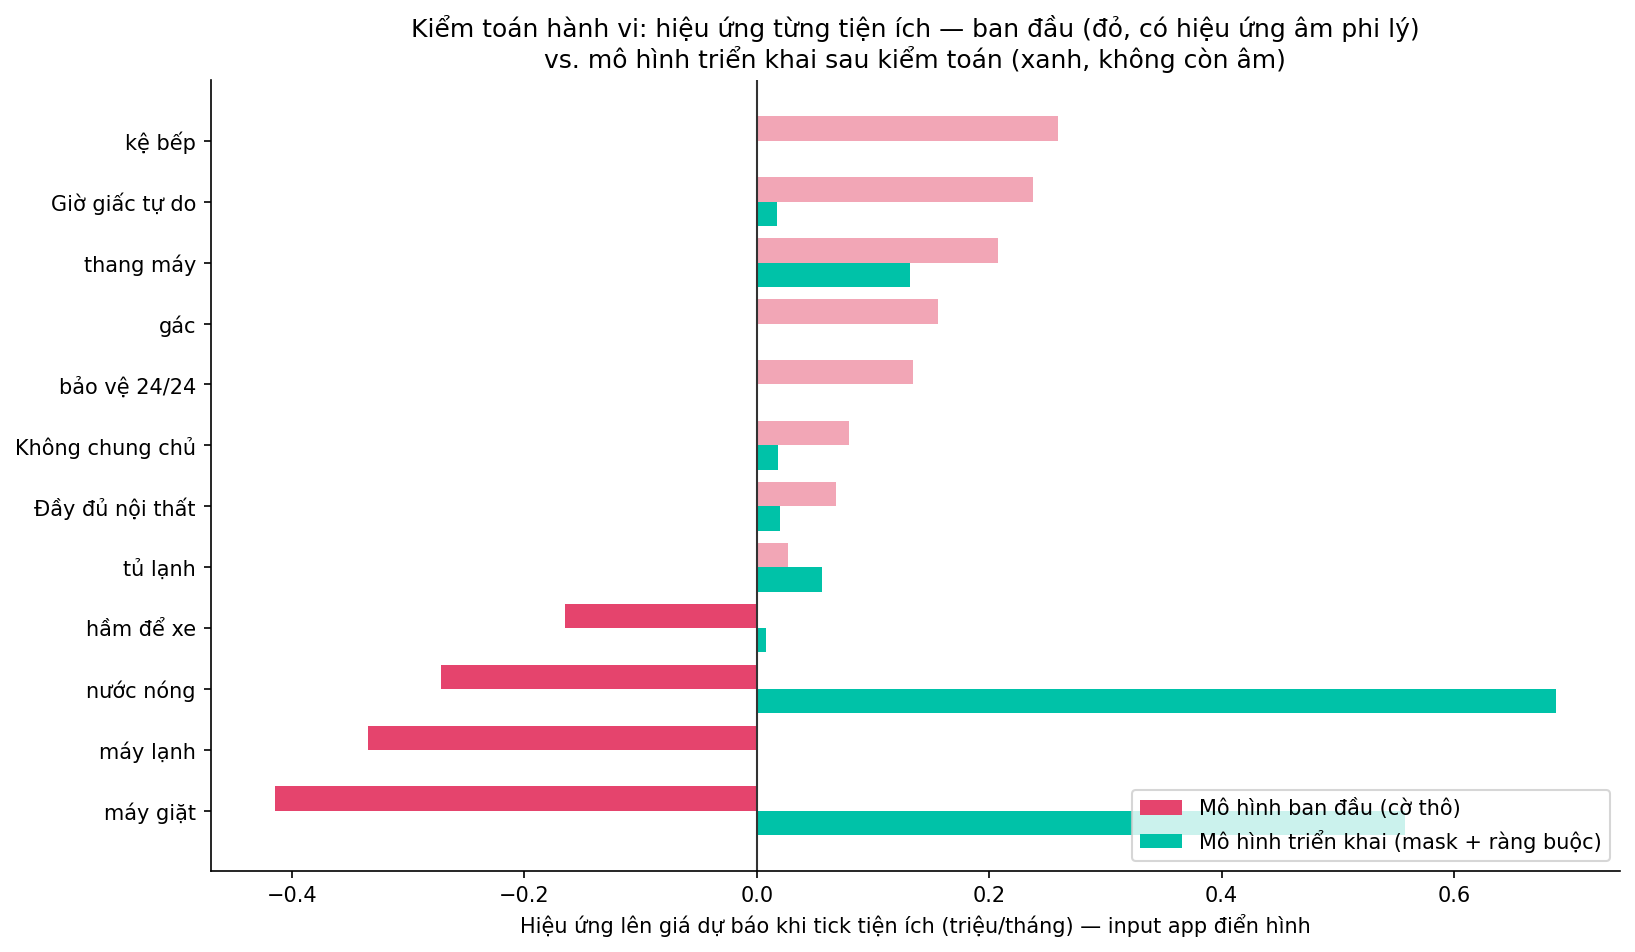
\includegraphics[width=0.92\textwidth]{audit_amenity_effects}
  \caption{Hiệu ứng tick từng tiện ích lên giá dự báo (input app điển hình) —
           mô hình ban đầu có 4 hiệu ứng âm phi lý (đỏ);
           mô hình triển khai sau kiểm toán không còn hiệu ứng âm nào (xanh)}
  \label{fig:audit_effects}
\end{figure}

\textbf{Phân tích đánh đổi — phần thảo luận quan trọng nhất của đồ án:}
\begin{itemize}[leftmargin=*, itemsep=3pt]
  \item \textbf{Làm sạch số giả tự nó cải thiện độ chính xác} (R\textsuperscript{2}
        $0.633 \to 0.671$ — thậm chí cao hơn cả Random Forest 0.664): các cờ chế tác là
        nhiễu kéo mô hình xuống. Điều này cũng cho thấy con số 0.633 ban đầu được ``bơm''
        một phần bởi trò nhận diện nguồn qua pattern cờ — không phải tín hiệu định giá thật.
  \item \textbf{Khoảng cách $0.671 \to 0.565$ là cái giá của việc từ chối tương quan
        phi nhân quả.} Tương quan ``quảng cáo tiện ích $\leftrightarrow$ giá rẻ'' là thật
        trong dữ liệu (nên giúp dự báo trên tập Test cùng phân phối), nhưng \textit{sai}
        đối với người dùng app — họ khai báo tiện ích thật của căn phòng, không phải
        hành vi đăng tin. Với kịch bản triển khai, mô hình ràng buộc là lựa chọn đúng.
  \item Lưu ý về tính nguyên sơ của Test: các biến thể trong kiểm toán được đo trên
        cùng tập Test để so sánh, nghĩa là Test không còn ``đúng 1 lần'' tuyệt đối
        cho mô hình cuối; tuy nhiên mọi lựa chọn cấu hình (siêu tham số, biến thể
        ràng buộc) đều dựa trên \textbf{Validation}, Test chỉ dùng để báo cáo.
\end{itemize}

\fbox{\parbox{0.97\textwidth}{\textbf{Quyết định D:} mô hình triển khai =
XGBoost trên dữ liệu \textbf{mask MNAR}, \textbf{bỏ \texttt{n\_features}},
\textbf{ràng buộc đơn điệu 12 cờ tiện ích} — Test R\textsuperscript{2} = 0.565,
MAE = 1.26 triệu/tháng, và \textbf{bảo đảm cấu trúc}: thêm tiện ích không bao giờ
làm giảm giá dự báo.}}

%% ============================================================
%%  SECTION 6 — KẾT LUẬN (Conclusion)  (số liệu: v2)
%% ============================================================
\section{Kết luận}
\label{sec:conclusion}

\subsection{Tóm tắt quá trình và kết quả}

Đồ án đã hoàn thành trọn vẹn quy trình Khoa học Dữ liệu (KDD) 6 bước:
thu thập 133.586 bản ghi từ 10 nguồn, tích hợp về lược đồ thống nhất,
làm sạch và phân tích khám phá, xây dựng và đánh giá 5 mô hình hồi quy,
kết thúc bằng ứng dụng demo Streamlit.

Mô hình triển khai \textbf{XGBoost} (sau kiểm toán MNAR + ràng buộc đơn điệu,
Mục~\ref{subsec:audit}) đạt:
\begin{itemize}[leftmargin=*, itemsep=2pt]
  \item \textbf{Test R\textsuperscript{2} = 0.565}; \textbf{Test RMSE = 1.895 triệu/tháng};
        \textbf{Test MAE = 1.26 triệu/tháng} — kèm \textbf{bảo đảm cấu trúc}:
        tick thêm tiện ích không bao giờ làm giảm giá dự báo
        (0 hiệu ứng âm, đơn điệu tuyệt đối trên app).
  \item Để tham chiếu: Random Forest chính xác hơn (Test R\textsuperscript{2} = 0.664), và
        biến thể XGBoost chỉ-làm-sạch-dữ-liệu (không ràng buộc) còn cao hơn nữa (0.671) —
        nhưng cả hai đều mang hiệu ứng tiện ích âm phi lý. Khoảng cách $\approx$0.10
        R\textsuperscript{2} là cái giá \textit{có chủ đích} của việc từ chối tương quan
        phi nhân quả để đổi lấy hành vi đúng cho app (Mục~\ref{subsec:audit}).
  \item Kích thước $\approx$0.86 MB, triển khai được trong giới hạn GitHub và app Streamlit.
\end{itemize}

\subsection{Bài học kinh nghiệm và ý nghĩa}

\begin{enumerate}[leftmargin=*, itemsep=5pt]
  \item \textbf{Diện tích và khu vực là yếu tố định giá mạnh nhất.}
        Feature Importance của cả RF lẫn XGBoost đều xếp \texttt{area}
        và \texttt{city}/\texttt{district} dẫn đầu sau khi loại \texttt{source}.

  \item \textbf{Nghịch lý Simpson là bài học về phân tích dữ liệu nghiêm túc.}
        Tương quan âm toàn cục giữa tiện ích và giá không phản ánh quan hệ nhân quả —
        đây là confounding variable do cấu trúc nguồn.
        Phát hiện này dẫn tới quyết định loại \texttt{source}
        (đánh đổi một phần độ chính xác nhưng đổi lại mô hình \textbf{trung thực và tổng quát hơn}).

  \item \textbf{Chỉ số tốt chưa đủ — phải kiểm thử hành vi và kiểm toán nguồn gốc dữ liệu.}
        Một hiệu ứng phi lý trên app (tick máy lạnh làm giá \textit{giảm}) được truy vết
        về tận dữ liệu thô, phát hiện \textbf{7/12 cờ tiện ích bị điền ngẫu nhiên ở bước
        tích hợp} ($\approx$97\% số dòng) — điều mà mọi chỉ số tổng hợp (RMSE, R\textsuperscript{2},
        CV) đều không phát hiện được. Bài học kép: (i) dữ liệu hợp nhất đa nguồn cần
        \textit{lưu vết nguồn gốc} (provenance) và phân biệt ``thiếu'' với ``không có''
        (MNAR); (ii) mô hình triển khai cho người dùng cần \textbf{đúng về hành vi}
        (ràng buộc đơn điệu), kể cả khi phải trả giá bằng chỉ số trên tập Test
        cùng phân phối với dữ liệu lỗi.

  \item \textbf{Các quyết định tiền xử lý phải được kiểm chứng bằng thực nghiệm, không chỉ lập luận.}
        Ba ablation study xác nhận:
        \begin{itemize}[itemsep=2pt]
          \item FE (tách khu vực từ địa chỉ) giảm RMSE 3.5--9.4\%;
                PCA không giúp ích với bộ dữ liệu này.
          \item Log-transform mục tiêu \textit{không} tăng hiệu năng theo tiêu chí RMSE/R\textsuperscript{2}
                và gây underweight phân khúc giá cao.
          \item Lọc ngoại lệ giảm RMSE 83.1\% trên vùng giá mục tiêu.
        \end{itemize}

  \item \textbf{Quan hệ phi tuyến mạnh.}
        Mô hình cây (R\textsuperscript{2} $\approx$ 0.57--0.66) vượt xa tuyến tính
        (R\textsuperscript{2} $\approx$ 0.19), xác nhận tương tác
        khu vực $\times$ diện tích không thể biểu diễn bằng hàm tuyến tính đơn giản.

  \item \textbf{Giới hạn bởi bias (không phải variance).}
        Learning curve cho thấy thêm dữ liệu cùng loại giúp ít —
        cần đặc trưng \textit{mới} (GPS, khoảng cách, NLP mô tả) để tăng R\textsuperscript{2}.
\end{enumerate}

\subsection{Hướng phát triển (Future Work)}

\begin{itemize}[leftmargin=*, itemsep=3pt]
  \item \textbf{Thu thập lại tiện ích thật} cho các nguồn đang thiếu
        (\texttt{chothuenhadattoanvn}, \texttt{github\_*}) và chạy lại toàn bộ
        so sánh 5 mô hình trên pipeline đã sửa MNAR — gỡ giới hạn
        ``tương quan hành vi đăng tin'' tận gốc thay vì bằng ràng buộc.
  \item \textbf{Đặc trưng vị trí không gian:} tọa độ GPS, khoảng cách đến trung tâm,
        tiện ích công cộng (trường học, bệnh viện, metro) — các nghiên cứu quốc tế
        cho thấy đây là yếu tố tăng R\textsuperscript{2} mạnh nhất.
  \item \textbf{Khai thác mô tả dạng văn bản:} NLP (TF-IDF, BERT) trên trường
        \texttt{description} để trích xuất tín hiệu giá (tầng, hướng, view, trang trí…).
  \item \textbf{Cân bằng dữ liệu địa lý:} thu thập thêm mẫu ngoài Hà Nội
        để mô hình đại diện tốt hơn cho các tỉnh thành khác.
  \item \textbf{Cập nhật định kỳ:} triển khai pipeline tự động cào và retrain
        hàng tháng, theo dõi data drift khi thị trường thay đổi.
  \item \textbf{Mô hình phức tạp hơn:} LightGBM, CatBoost, hoặc deep learning
        (TabNet) nếu bổ sung được đặc trưng GPS và văn bản.
\end{itemize}


\newpage
%% ============================================================
%%  TÀI LIỆU THAM KHẢO (đặt cuối báo cáo)
%%  Tiêu đề "Tài liệu tham khảo" do babel vietnamese đặt (\refname)
%% ============================================================
\begin{thebibliography}{9}
  \bibitem{rosen1974hedonic}
    Rosen, S. (1974).
    \textit{Hedonic prices and implicit markets: Product differentiation in pure competition.}
    Journal of Political Economy, 82(1), 34--55.

  \bibitem{decock2011ames}
    De Cock, D. (2011).
    \textit{Ames, Iowa: Alternative to the Boston Housing Data as an End of Semester Regression Project.}
    Journal of Statistics Education, 19(3).

  \bibitem{yilmaz2022rental}
    Yılmaz, İ., \& Yakut, E. (2022).
    \textit{Predicting rental prices using machine learning: A case study.}
    International Journal of Applied Mathematics, Electronics and Computers, 10(2).

  \bibitem{github_hcm_housing}
    GitHub contributors. (2022--2024).
    \textit{Vietnam Housing Price Prediction (open-source repositories)}.
    Truy cập tại: \url{https://github.com/topics/vietnam-housing}
\end{thebibliography}


\end{document}
